\chapter{Results}\label{chap:results}

This chapter will present the outcomes of the design and development phase.
First, the artifact is presented from a user's point of view, showcasing functionality with screenshots.
Then, the artifact's design will be presented from an architectural view, and the protocol will be presented last.\\

The results will also present the measures taken for making the \gls{open source} project viable, and something a developer community may want to develop and maintain further.\\

Evaluation of the results is presented later, in \cref{chap:evaluation}.\\

An overview of the results can be previewed in the informal \cref{fig:results-overview}.

\begin{figure}[H]  % order of priority: h here, t top, b bottom, p page
  \centering
  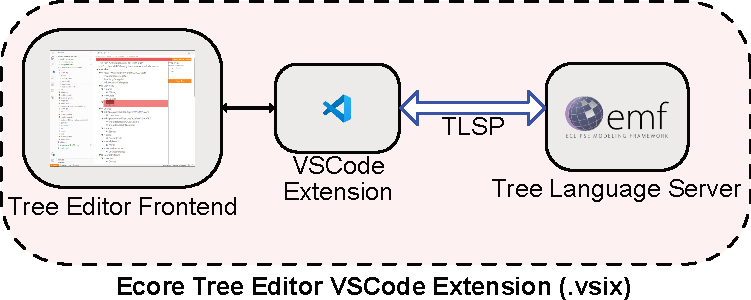
\includegraphics[width=\textwidth]{figures/result_overview.pdf}
  \caption[Overview of Results]{Informal diagram of the results, showing the main components.}\label{fig:results-overview}
\end{figure}

\section{Software Artifact: Tree Editor Extension for Ecore in Gitpod}

This is of interest for a stakeholder, and someone aiming to do further research on this design.

The output of the development phase is an artifact which is a \gls{VSCode} extension.
The artifact is a \texttt{.vsix} file, and can be installed in a \gls{Gitpod} workspace.
The following results are from \gls{Gitpod} using \gls{VSCode} as the editor frontend, not \gls{Theia}\footnote{VSCode is the default for Gitpod, instead of Theia~\cite{georgetsiolisMenuEntryGitpod2019,svenefftingeProductRoadmapQ1}.}.
One way to install it\footnote{The ``best'' way is to publish the extension to OpenVSX, and search for it in the extensions panel.}, is to upload the \texttt{.vsix} file to the workspace, right clicking on it and selecting ``Install Extension VSIX''.
When installed in the \acrshort{IDE}, it is shown in the extensions panel as \textit{Ecore Tree-editor}, shown in \cref{fig:gitpod-ext-installed}.

\begin{figure}[H]  % order of priority: h here, t top, b bottom, p page
  \centering
  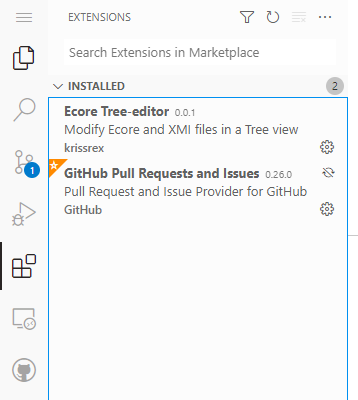
\includegraphics[width=0.6\textwidth]{figures/gitpod-vscode-extensions-installed.png}
  \caption[Tree Editor Extension installed in Gitpod]{The extension is installed as \textit{Ecore Tree-editor} in Gitpod with VSCode.}\label{fig:gitpod-ext-installed}
\end{figure}

\subsection{Custom Editor}

This extension adds a new Custom Editor, which is automatically opened when the user opens a \texttt{.ecore}, \texttt{.genmodel} or \texttt{.xmi} file.
The model file is loaded and transformed by the extension, and presented as a tree to the user.

\begin{figure}[H]  % order of priority: h here, t top, b bottom, p page
  \centering
  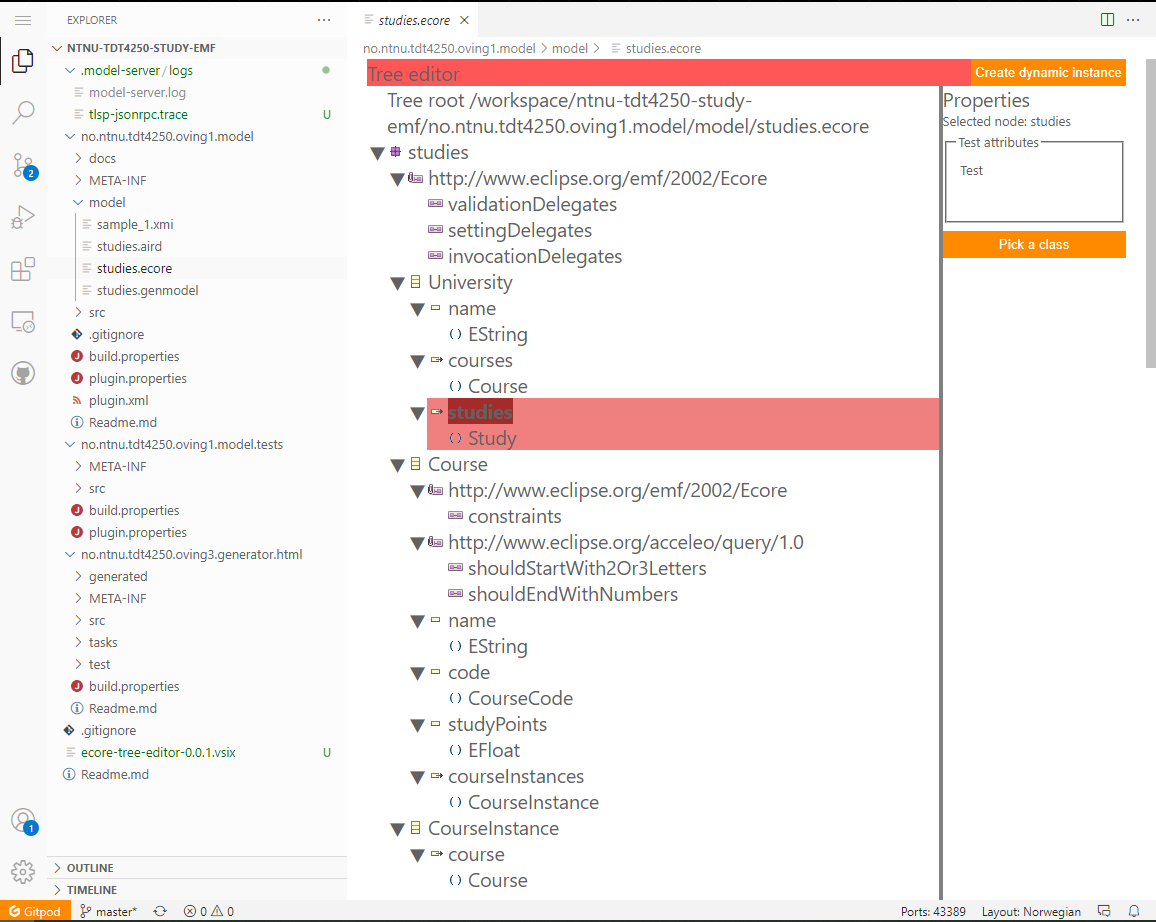
\includegraphics[width=\textwidth]{figures/gitpod-vscode-ecore-editor-studyemf.png}
  \caption[Tree Editor Extension showing studies.ecore]{The Tree Editor Extension has opened a Custom Editor for the \texttt{studies.ecore} file.}\label{fig:gitpod-ext-tree-ecore}
\end{figure}

\paragraph{Example model}
An \gls{Ecore} model made in \gls{TDT4250} in 2019 has been used as an example to demonstrate the artifact.
The \texttt{.ecore} file is opened in \cref{fig:gitpod-ext-tree-ecore}.
This figure shows three columns, from left to right: the default \gls{VSCode} file explorer, the custom editor's master layout (tree structure), and the custom editor's detail layout (properties sheet).

\paragraph{Action bar}
There is also a red action bar at the top, with an orange action button to create a new dynamic instance.
The action buttons shown will vary, depending on what the selected node is.
The orange color of the button is coming from the color theme of the \gls{VSCode} editor.
With a dark theme, this action button could be blue, for example.

\paragraph{Master layout}
The master layout can show multiple roots.
In this document,  single root is shown for the ``studies.ecore'' file.
The root node is a ``studies'' package, with children displayed below.
This node has a label, ``studies'', and a specific icon indicating it is a package --- the purple box with a cross.
The icons used are the same ones used in \gls{Eclipse} for the Sample Reflective Ecore Editor (see \cref{sec:sample-reflective-editor}), and depend on the type of node.

Clicking the black triangle next to a node will collapse it, hiding its children and rotating the triangle 90 degrees counter-clockwise.

Inside the master layout, a node is selected in dark red, with the label ``studies''.
Its child node ``Study'' is also highlighted, in a lighter red.
(Note that the colors of selected nodes were arbitrarily chosen during development, and could be changed to give more contrast with the node's label.)
A node can be selected by clicking on it, and holding \texttt{ctrl} will add to the selection, allowing multiple nodes to be selected.

Dragging a node in the hierarchy and dropping it on a node, should change this node's parent.
Right clicking a node will open a context menu, with the possible children nodes to add.
Dropping a node on an invalid parent will be prevented, by using a hierarchy schema, and indicated by changing the mouse cursor to a ``forbidden'' icon\footnote{Note that drag-and-drop and node creation are not currently implemented, only accounted for by the design, by using a hierarchy schema.}.


\paragraph{Detail layout}
The detail layout has a property sheet, currently showing a unfinished example form.
This layout should use the \textit{JSON-Forms} library to render properties, based on the node's properties and a \textit{UI schema} for that node type.


\subsection{IDE Commands}

The extension also provides Commands to \gls{VSCode}.
These are actions that can be invoked at any time.
The student can invoke them from the Command Palette\footnote{Press \texttt{F1}, or \texttt{ctrl + shift + P} (command on mac), or \texttt{Menu $\rightarrow$ View $\rightarrow$ Command palette}} by typing ``Ecore'' or another part of the command's name.
A screenshot is shown in \cref{fig:gitpod-ext-newmodel}, with a command to create a new model file.
This file will have the minimum \acrshort{XMI} contents required for a blank model.

\begin{figure}[H]  % order of priority: h here, t top, b bottom, p page
  \centering
  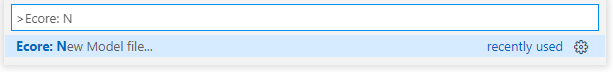
\includegraphics[width=\textwidth]{figures/gitpod-vscode-newmodel.png}
  \caption[Tree Editor Extension Custom Commands]{The Tree Editor Extension adds custom commands to the Command Palette. One of them is shown here, named \textit{Ecore: New Model file\ldots}.}\label{fig:gitpod-ext-newmodel}
\end{figure}

\subsection{Genmodel and Model Instance}

The editor can open a \texttt{.genmodel} file or a \texttt{.xmi} model dynamic instance file as well.
The genmodel is shown in \cref{fig:gitpod-ext-genmodel}, and the dynamic instance in \cref{fig:gitpod-ext-dynamic}.
This will show two roots in the editor, as the original \texttt{.ecore} model is related to the opened file.
One root is the genmodel (or model dynamic instance), and the other root is the study model.

The GenModel editor is not specialized, so it renders the tree as any other \gls{Ecore} model.

\begin{figure}[H]  % order of priority: h here, t top, b bottom, p page
  \centering
  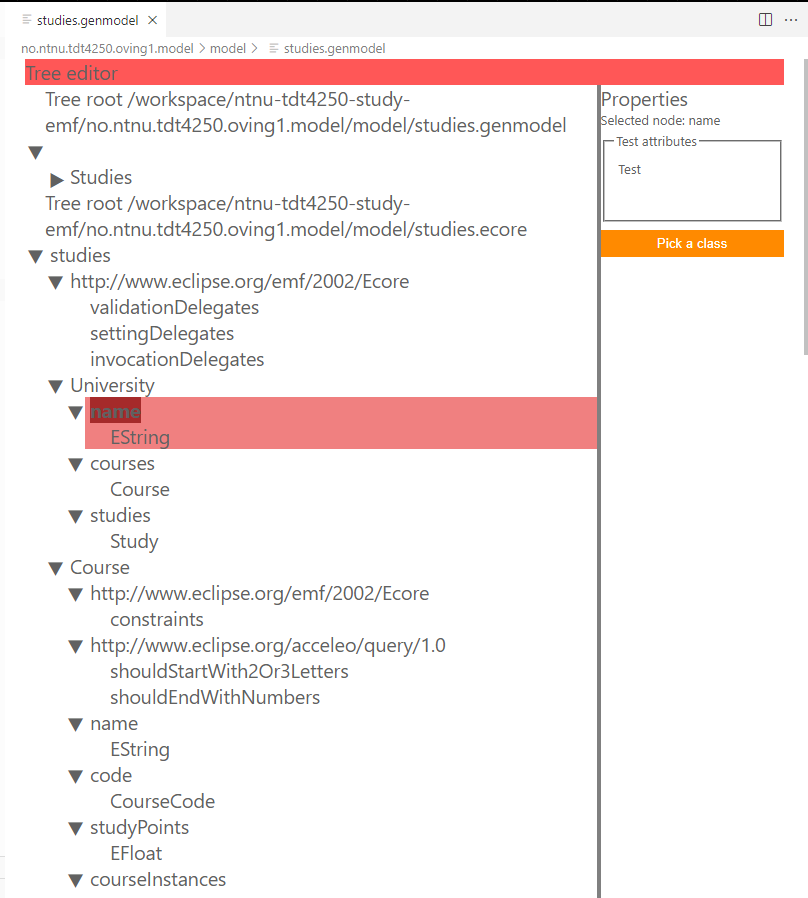
\includegraphics[width=\textwidth]{figures/gitpod-vscode-genmodel.png}
  \caption[Tree Editor Extension showing studies.genmodel]{The Tree Editor Extension with the \texttt{studies.genmodel} file open. It has two roots, the GenModel and the model. The GenModel is collapsed/hidden at the ``Studies'' node.}\label{fig:gitpod-ext-genmodel}
\end{figure}

\begin{figure}[H]  % order of priority: h here, t top, b bottom, p page
  \centering
  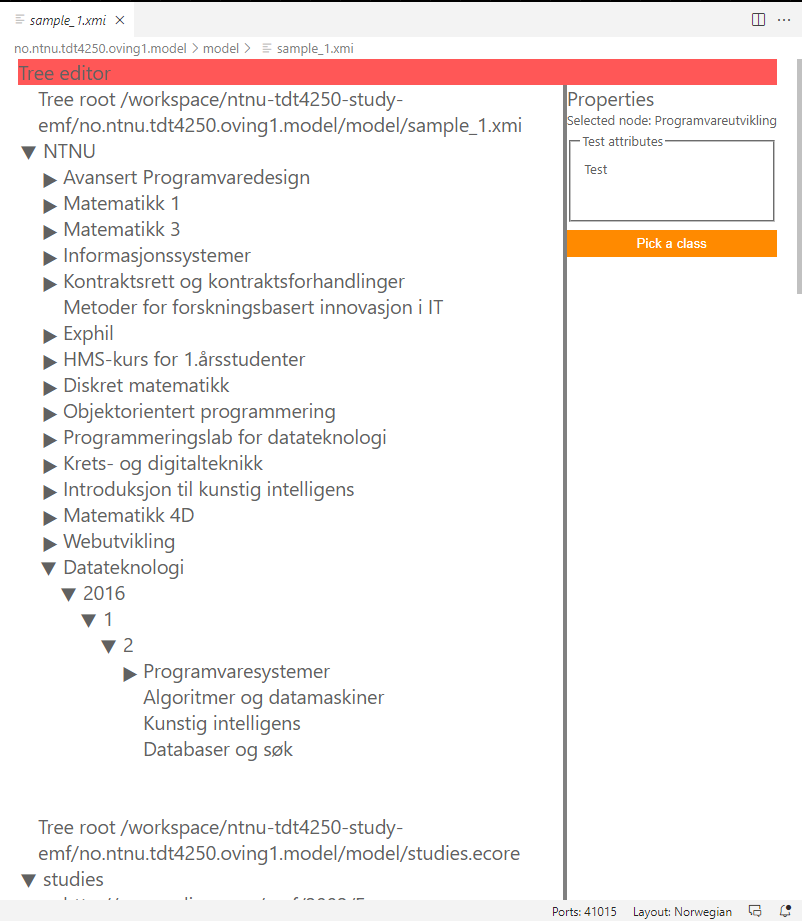
\includegraphics[width=\textwidth]{figures/gitpod-vscode-xmi-study-instance.png}
  \caption[Tree Editor Extension showing a dynamic instance]{The Tree Editor Extension with the \texttt{sample\_1.xmi} dynamic instance open. This is data that conforms to the model defined in \texttt{studies.ecore}.}\label{fig:gitpod-ext-dynamic}
\end{figure}


\subsection{Configuration and Logging}

The extension has configuration options that a user can set.
One such option is the logging level, a threshold to hide log messages in the log panel.
The extension can also log internal events and messages to a Output panel in \gls{VSCode}, for the user to debug and identify extension errors.
This is mostly useful for extension developers, not students.
But it works as an example of using configuration options.
It is identified that using configurations will be needed.
The configuration and output panel are shown in \cref{fig:gitpod-ext-config-log}.

\begin{figure}[htbp]  % order of priority: h here, t top, b bottom, p page
  \centering
  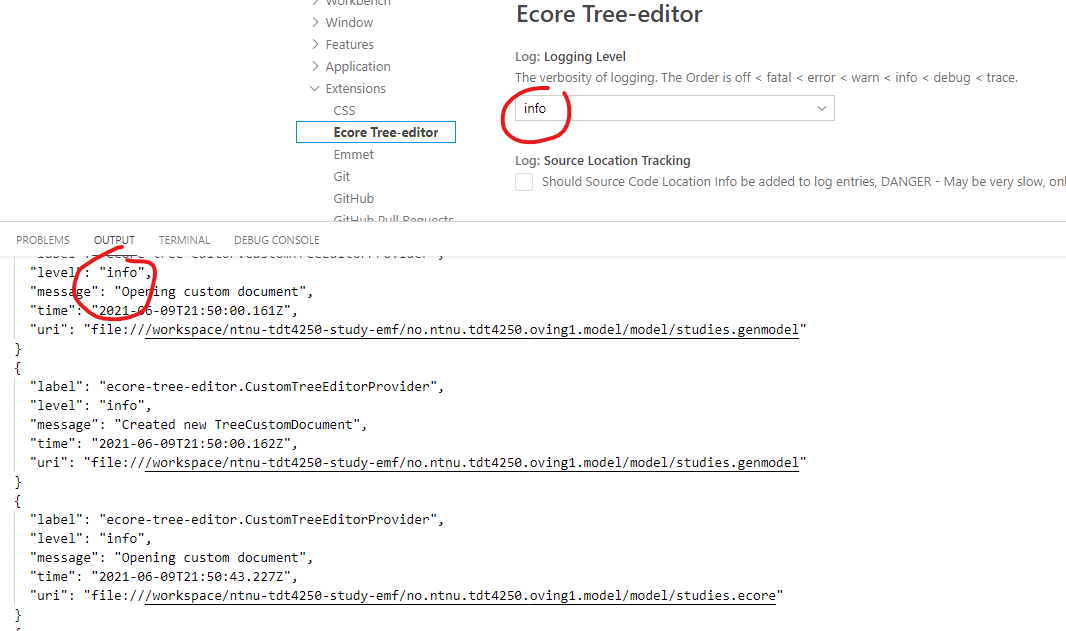
\includegraphics[width=\textwidth]{figures/gitpod-vscode-config-and-logging.png}
  \caption[Tree Editor Extension with configuration and logging]{The Tree Editor Extension adds configuration options to the \gls{VSCode} settings menu, shown in the top right.
  The extension also adds log outputs to a Output panel.
  The figure is annotated with two red circles.
  The upper circle is indicating the configuration option to filter the output based on log level.
  The lower circle is highlighting that same log level from a message in the output panel.}\label{fig:gitpod-ext-config-log}
\end{figure}


\iffalse{
% * Steps:
% 1. Sign up to Gitpod.io with GitHub user
% 2. Go to Settings. Set default IDE as VSCode. (It will be the default soon % % https://github.com/gitpod-io/gitpod/issues/3989#issuecomment-822246441)
% 3. Open %https://gitpod.io/#https://github.com/krissrex/ntnu-tdt4250-study-emf % to get a Workspace in gitpod with an EMF project. The Tree Language Server does % not support multi-workspace.
% 4. Build the extension locally to obtain a .vsix file (or download a build from % somewhere)
% 5. Upload the .vsix to the project workspace by drag-and-drop.
% 6. Right-click the .vsix file in VSCode/Gitpod, select "Install Extension VSIX".
% 7. Wait for "Completed installing Ecore Tree-editor extension from VSIX" popup % in bottom right corner.
% 8. Open folder with models: "no.ntnu.tdt4250.oving1.model/model"
% 9. Click model file: "studies.ecore"
% 10. Click genmodel file: "studies.genmodel"
% 11. Click dynamic instance file: "sample_1.xmi"
}
\fi

\FloatBarrier % Prevent figures running into the next section

\section{Design Artifact: Tree Document Model}

A central design result is the constructs used to represent trees in an editor.
These constructs are referred to as the \textbf{domain model} or simply \textbf{model} in this section (not to be confused with an \acrshort{Ecore} model).
This representation is what the frontend presents to a user, and what the extension and server is using to communicate over \acrfull{TLSP}.
Knowing this model is essential for communicating how the design works.
This is because it is used as the ``ubiquitous language'' formed by Domain-driven design (see \cref{sec:ddd} and \cite{evansDomaindrivenDesignTackling2004}).
Note that \textbf{the domain model is generic for all trees and unaware of \acrshort{EMF}}.
This is because it aims to be a domain model for the \acrshort{TLSP}, reuseable for other use cases than \acrshort{EMF} editing.
This section will explain where some of the names come from, and what these data structures look like.\\

\subsection{Borrowed Terms}

\paragraph{Trees}
When words like tree, node, root and children are used, they refer to the concepts for tree structures described in \cref{sec:tree-structures}.
A tree has exactly one root.
The root can have nodes as children, and these can have children again.
A node has a name and an icon that can represent it in a hierarchical tree structure.

\paragraph{Icon}
An icon is a visual representation --- a picture, illustration, symbol --- that represents some information about a node.
An icon can show how one node differs from another, like what type it is, or it can show if a node is invalid or not.

\paragraph{DataUri}
This is a more technical term.
The trees will be displayed on the web, with icons.
A way to store icons as text is using the HTML data-uri scheme.
It is just text, but has a semantic meaning.
When set as the image source in a web browser, it will be displayed as a picture.
A data-uri starts with a prefix which specifies the scheme, the content type and the encoding, for example: \lstinline|data:image/gif;base64,|.
Then, it is followed by the encoded image.

\paragraph{Document}
Because this is for an editor, the concept of documents are borrowed from \gls{VSCode}.
A document is the editor's representation of a file that the user wants to modify.
When a editor window is open in an \acrshort{IDE}, this editor shows a single document.
The document can be opened, modified, saved, renamed and so on.


\subsection{The Domain Model}

The domain model is specified in this thesis by using \gls{TypeScript}, but it can be translated to other languages, such as java.\\

A brief summary of the more exotic features of \gls{TypeScript} may be helpful for the reader:
Note that the `?' means optional or nullable.
\gls{TypeScript} can also ``alias'' types, meaning a new type can be defined by simply renaming an existing type.
This can put more meaning into types like \texttt{string} and \texttt{number}, especially when they are reused in multiple places.
Some builtin interfaces are used, like \texttt{Array} (a list) and \texttt{Record} (an object, or dictionary/map-like structure with keys and values).\\

The domain model will now be presented.
It consists of the following elements: \texttt{TreeDocument}, \texttt{TreeRoot}, \texttt{TreeNode}, \texttt{NodeIcon}, \texttt{IconConfiguration}, \texttt{HierarchyConfiguration}, \texttt{Action}, \texttt{ActionEvent}, \texttt{ActionConfiguration} and \texttt{EditorState}.
It also defines the following aliases for strings: \texttt{ActionId}, \texttt{IconDataUri}, \texttt{NodeId} and \texttt{NodeType}.
These concepts are explained below.

\paragraph{TreeDocument}
The main data structure is the \texttt{TreeDocument}, in \cref{lst:result-tree-document}.
This holds a list of \texttt{TreeRoot}s.
A document can have multiple roots, because there can be related trees.
For example in \acrshort{EMF}, the \texttt{.genmodel} file has a related \texttt{.ecore} file.
Opening the GenModel would also show the \gls{Ecore} model, in an editor with two roots.

\begin{lstlisting}[language=Typescript, label={lst:result-tree-document}, caption={[TreeDocument]TreeDocument TypeScript code.}]
interface TreeDocument {
  roots: Array<TreeRoot>;
}
\end{lstlisting}

\paragraph{TreeRoot}
The \texttt{TreeRoot} in \cref{lst:result-tree-root} holds references to the tree's root node.
It also holds the configurations for how the nodes should be given icons, what actions a user can perform on the nodes, and what a valid node hierarchy looks like.
The actions, hierarchy and icons use the \texttt{type} property of \texttt{TreeNode} to enforce this.
The \texttt{TreeRoot} has an id as well, to separate it from other roots.
This id must be unique inside the TreeDocument.\\

A \texttt{TreeRoot} does not require a root node, for example in the case the \texttt{TreeRoot} was just created or the node was deleted.

\begin{lstlisting}[language=Typescript, label={lst:result-tree-root}, caption={[TreeRoot]TreeRoot TypeScript code.}]
interface TreeRoot {
  id: string;
  rootNode?: TreeNode;
  actions: ActionConfiguration;
  hierarchy: HierarchyConfiguration;
  icons?: IconConfiguration;
}
\end{lstlisting}


\paragraph{TreeNode}
For representing the nodes themselves, there is the \texttt{TreeNode} in \cref{lst:result-tree-node}.
It has an id that is unique in the \texttt{TreeDocument}.
The id is a string, but aliased to \texttt{NodeId} in \gls{TypeScript}.\\

Next, the \texttt{TreeNode} has a \texttt{type}, which is very important.
This type is a string, for example ``EClass'' or ``EAttribute'', and decides the icon, the allowed child nodes, and the possible actions a user can perform on this node.
The string is aliased as \texttt{NodeType} in the model.\\

The \texttt{name} is what shows up in the hierarchical tree structure when presented to the user.
It also reflects a property the user can edit.
The name can for example be ``MyClass'', ``Organization'' or ``NTNU''.\\

To help inform the user what a node represents, the \texttt{documentation} property can hold a help string.
The user interface could show this on hover, or when a node is selected in a designated help area.\\

The \texttt{TreeNode} holds instances of other \texttt{TreeNode}s in the \texttt{children}-property.
This is what enables the tree structure to be represented.\\

Sometimes, a node can be special, for example invalid.
To indicate this, the optional \texttt{iconOverride} can specify a new icon instead of the one from the \texttt{TreeRoot}'s icon configuration.\\

The last property is the \texttt{EditorState}.
This has the properties \texttt{selected} and \texttt{collapsed}, used to hold presentation information about the node.
Being collapsed means that the children are not shown.

\begin{lstlisting}[language=Typescript, label={lst:result-tree-node}, caption={[TreeNode]TreeNode TypeScript code.}]
interface TreeNode {
  id: NodeId;
  type: NodeType;
  name?: string;
  documentation?: string;
  children: Array<TreeNode>;
  iconOverride?: IconDataUri | NodeIcon;
  editorState?: EditorState;
}
\end{lstlisting}


\paragraph{Action}
As mentioned, a user can perform actions.
These can be validating an \gls{Ecore} model, creating a new dynamic instance, and so on.
This is represented by an \texttt{Action} in \cref{lst:results-action}.
The purpose of the \texttt{Action} is to show the user something they can perform, but only contain enough information so it can be sent back to the Tree Language Server to be performed there.
Essentially, an \texttt{Action} is like a reference to a procedure on the server.\\

The action has an \texttt{id}, which is unique in the \texttt{TreeRoot}.
This is what the server uses to know which procedure should be executed.
The \texttt{name} and optional \texttt{icon} are for presenting the \texttt{Action} to the user.

\begin{lstlisting}[language=Typescript, label={lst:results-action}, caption={[Action]Action TypeScript code.}]
interface Action {
  id: ActionId;
  name: string;
  icon?: IconDataUri;
}
\end{lstlisting}

\paragraph{ActionConfiguration}
The list of all \texttt{Action}s live under the \texttt{TreeRoot}, inside the \texttt{ActionConfiguration}.
The intention is that the user is presented with an action bar, or other list of actions, which can change depending on the selected \texttt{TreeNode}.
This \texttt{ActionConfiguration} in \cref{lst:result-action-config} also specifies what actions are always shown in such an action bar, in the \texttt{defaultActionbarActions}.\\

The mapping of \texttt{ActionId}s to lists of \texttt{NodeType}s in \texttt{nodeActions} is used when a node is selected.
Each id can be examined to see if it supports the given \texttt{NodeType}.
The type is supported if it is present in that \texttt{ActionId}'s list.


\begin{lstlisting}[language=Typescript, label={lst:result-action-config}, caption={[ActionConfiguration]ActionConfiguration TypeScript code.}]
interface ActionConfiguration {
  availableActions: Array<Action>;
  defaultActionbarActions?: Array<ActionId>;
  nodeActions?: Record<ActionId, Array<NodeType>>;
}
\end{lstlisting}


\paragraph{ActionEvent}
When the user triggers an action from the frontend, it is sent as an \texttt{ActionEvent} to the server.
The \texttt{ActionEvent} is shown in \cref{lst:result-action-event}.
To reference which \texttt{Action} was triggered, the \texttt{ActionId} is set in the \texttt{action} property.
The server may also want to know what \texttt{TreeRoot} the selected node was in, at the time of triggering the action.
Because actions can operate on specific nodes, like creating a new dynamic instance in \acrshort{EMF}, the currently selected \texttt{TreeNode}'s id are set as the \texttt{targetNodes}.

\begin{lstlisting}[language=Typescript, label={lst:result-action-event}, caption={[ActionEvent]ActionEvent TypeScript code.}]
interface ActionEvent {
  targetNodes?: Array<NodeId>;
  action: ActionId;
  targetRoot: TreeRoot;
}
\end{lstlisting}

\paragraph{NodeIcon and IconDataUri}
A \texttt{TreeNode} and an \texttt{Action} can have icons.
There are also icons in the \texttt{TreeRoot}'s \texttt{IconConfiguration}.
A single image is specified as \texttt{IconDataUri}, which is just an alias to a string type.\\
However, for more complex icons like the nodes', an editor may want to layer or alter the icons.
It could be to add multiplicity information, validity state, or other variants of an icon.
This is supported through composition with the \texttt{NodeIcon}.
It defines a list of \texttt{IconDataUri}s, which are drawn from bottom to top, stacked on each other.

\paragraph{HierarchyConfiguration}
The final element presented is the \texttt{HierarchyConfiguration} in \cref{lst:result-hierarchy-config}.
The \texttt{roots} specify what is allowed to be a \texttt{TreeRoot}'s \texttt{rootNode}.
For example, ``EPackage'' could be such a \texttt{NodeType}.\\

The \texttt{allowedChildren} specifies a mapping between a parent's \texttt{NodeType} and its possible children's \texttt{NodeType}.
This is designed with node creation an drag-and-drop in mind.
A mapping could for example be ``EClass'' to ``EAttribute'', ``EAnnotation'' and ``EReference''\footnote{This mapping is an example, and not complete.}.

\begin{lstlisting}[language=Typescript, label={lst:result-hierarchy-config}, caption={[HierarchyConfiguration]HierarchyConfiguration TypeScript code.}]
interface HierarchyConfiguration {
  roots: Array<NodeType>;
  allowedChildren: Record<NodeType, Array<NodeType>>;
}
\end{lstlisting}


\section{Design Artifact: Architecture for Tree Language Server Systems}

The software architecture may be of interest to developers of tree editors and similar kinds of \gls{VSCode} extensions.
There is potential to directly reuse components from this design.

\subsection{Architecturally Significant Requirements}
The high level software architecture for the tree editor was shaped mainly by three \acrfullpl{ASR}.
The editor must be a \gls{VSCode} extension, the tree viewer must use the \gls{VSCode} Custom Editor \gls{API}, and the extension must reuse \acrshort{EMF} java code and the EMF.Cloud Model Server.
This results in a system of three main components: a \textit{Tree editor frontend}, a \textit{Tree editor extension} and a \textit{Tree Language Server}.

Another \acrshort{ASR} is that the model may change, and the rest of the system must respond and be updated.
Therefore, a bi-directional communication between components is established, and an event driven architecture is used.
The communication is isolated and standardized in a protocol, called the \textit{Tree Language Server Protocol} (\acrshort{TLSP}).
This protocol is presented in detail in \cref{sec:tlsp}.


\subsection{Changes from pre-project}
From the pre-project, the high level architecture (see \cref{fig:pre-project-tree-editor-architecture}) changed mainly by avoiding the EMF.Cloud Model Server as a separate running process, and is now embedded inside the Tree Language Server~\cite[p.~49]{rekstadModelingEnvironmentCloud2020}.\\

On the code level, only the extension code and tree document model are similar.
The tree document model has changed to accommodate multiple roots, by introducing the \textit{TreeRoot} and moving the \textit{ArchitectureSchema} and \textit{IconConfiguration} as children of these root, instead of the \textit{TreeDocument}.
This allows configurations to be different on a per-root basis, which is needed when for example opening both a GenModel and \gls{Ecore} model in the same document.\\

The frontend is different from the pre-project prototype by using the \textit{Vue.js} framework, and implementing actual features.
The pre-project was only an example viewer, not communicating with the extension.\\

For the EMF.Cloud Model Server, this is now bundled inside the Tree Language Server, instead of a separate component.
The pre-project used \gls{REST} to communicate, while now it happens in java by using the classes of the EMF.Cloud Model Server, then relaying the answers over \acrshort{TLSP}.
The pre-project did not implement any real logic inside the server either.


\subsection{System explanation}
This section will explain the software architecture through a series of diagrams called the \textit{C4 Model} (Context, Container, Component, Code)~\cite{simonbrownC4ModelVisualising}.
This is a top-down approach where one ``zooms'' in on the system components, so the wider context is clear.


\subsubsection{Context}
At a high level, the system has students interacting with \gls{Gitpod}.
The developed system runs inside \gls{Gitpod} as an extension.
This is illustrated in \cref{fig:gitpod-system-context}.
The student use \gls{Gitpod} as a development environment, where they use the \acrshort{IDE}, change files in a Workspace, and runs programs in a terminal.
\Gls{Gitpod} uses \gls{git} to retrieve the student's code from \gls{GitHub}, and pushes changes back to it.

When a Student wants to install an extension to the \acrshort{IDE} in \gls{Gitpod}, it can either let the Student upload an extension file, or search the publicly available extensions in the OpenVSX extension registry.
The instantiated artifact from this thesis could be uploaded to OpenVSX.


\begin{figure}[H]  % order of priority: h here, t top, b bottom, p page
  \centering
  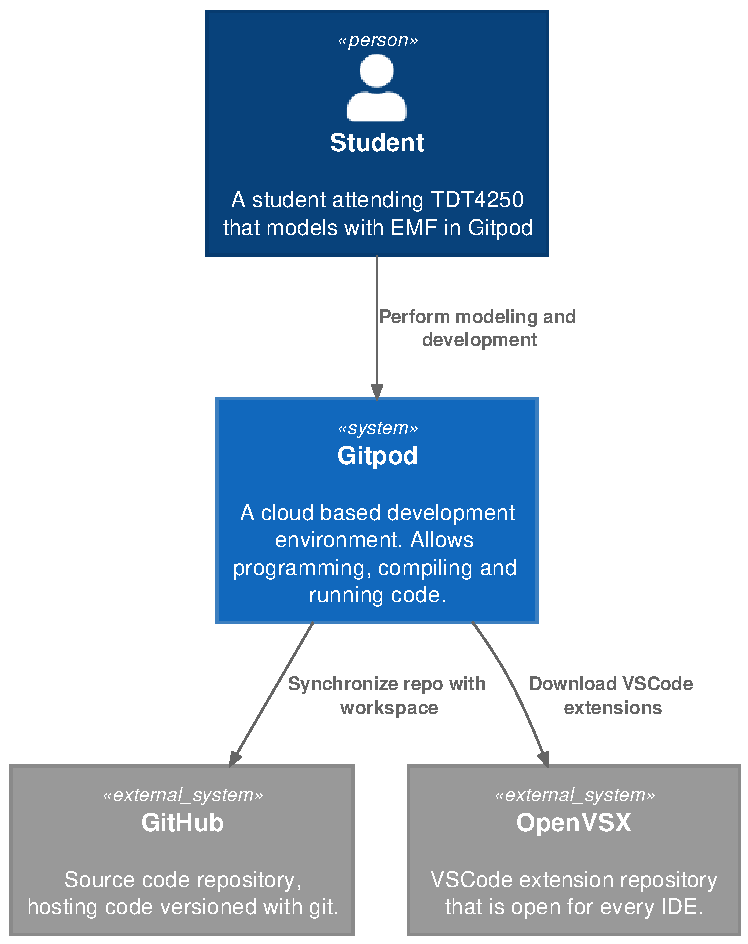
\includegraphics[width=\textwidth]{figures/plantuml/Gitpod_context.pdf}
  \caption[System context diagram for Gitpod]{A system context diagram for Gitpod. The extension will run inside the Gitpod service, used by a student to do modeling and developing. Gitpod uses git to synchronize code with GitHub. The extensions in Gitpod are downloaded from a service called OpenVSX.}\label{fig:gitpod-system-context}
\end{figure}

\subsubsection{Containers}

Inside the \gls{Gitpod} system, there is a \acrshort{IDE}, the \textit{Ecore Tree Editor Extension} from this thesis, and the Workspace.
This is shown in \cref{fig:gitpod-container-diagram}.
The \acrshort{IDE} can be \gls{Theia} or \gls{VSCode}.
This \acrshort{IDE} is responsible for providing the user interface to the student.
It also has the responsibility of installing and activating the extension.
The extension runs in the environment provided by the Workspace.
For example, the operating system and the available programs are provided by the Workspace, as well as the student's project files.
If the extension wants to run a java program, the Workspace must have a Java Runtime installed.

\begin{figure}[H]  % order of priority: h here, t top, b bottom, p page
  \centering
  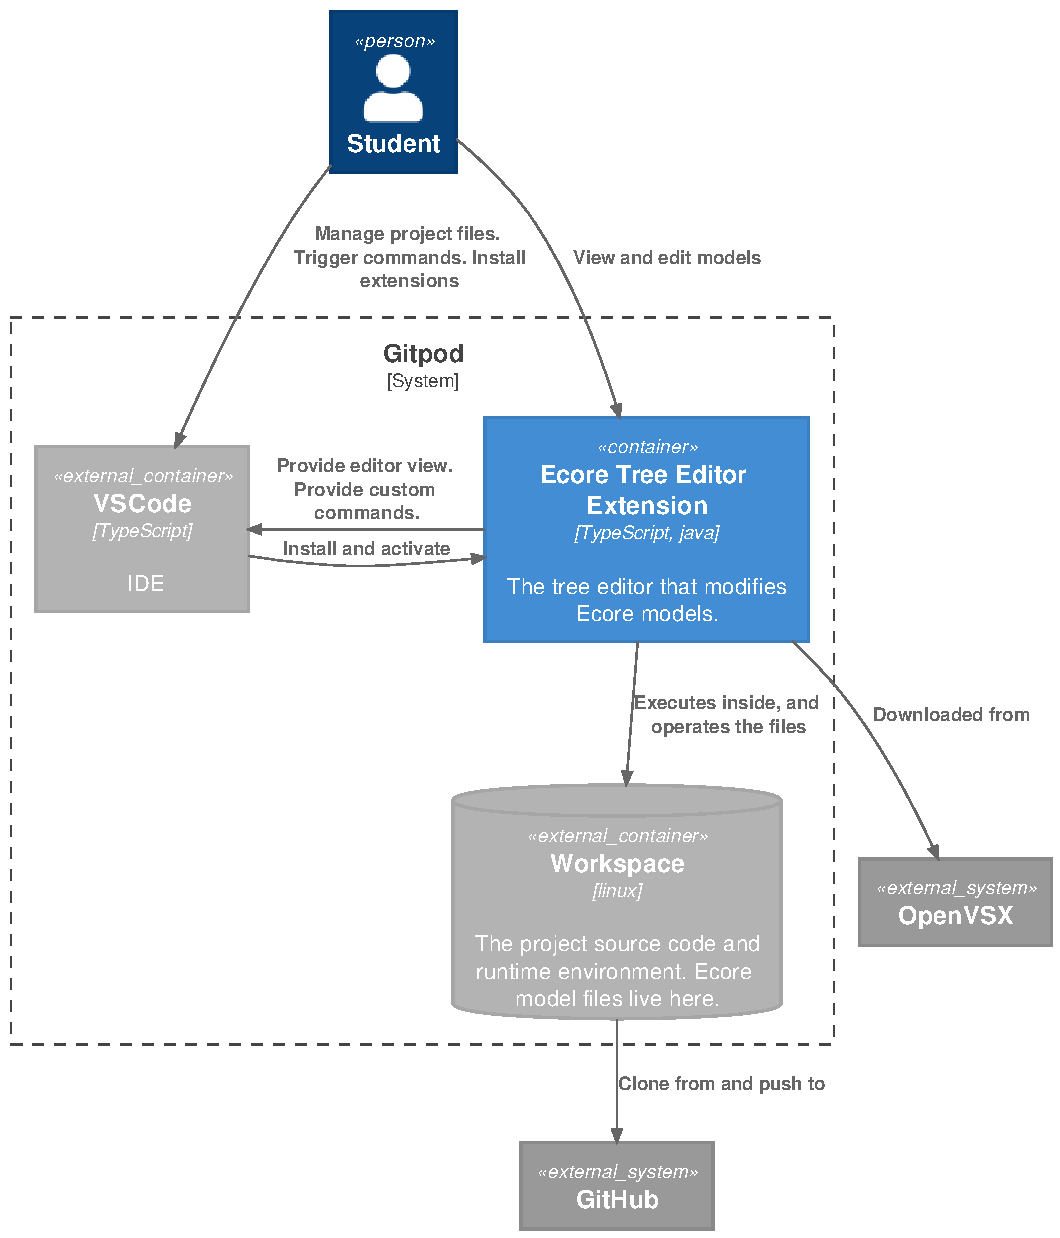
\includegraphics[width=\textwidth,height=\textheight,keepaspectratio]{figures/plantuml/Tree_Editor_Extension_container.pdf}
  \caption[Gitpod container diagram]{Container diagram for gitpod. The Gitpod system from \cref{fig:gitpod-system-context} is expanded to show its internal components. The \acrshort{IDE} used by Gitpod is \gls{VSCode}.
  The student will interact with VSCode, and install the Ecore Tree Editor Extension created from this thesis.
  This extension will also provide a user interface, which the student uses for modeling.
  This extension reads files from the Gitpod workspace, and uses the runtime provided by the workspace such as a Java Runtime Environment.}\label{fig:gitpod-container-diagram}
\end{figure}


\subsubsection{Components}

The Ecore Tree Editor Extension itself consists of three main components.
It is the \textit{Tree editor extension} (or simply ``extension''), which integrates with \gls{VSCode} or \gls{Theia}.
Then there is the \textit{Tree editor frontend} (or ``frontend''), which provides a user interface with the hierarchical tree structure, labels and icons to the student.
The last component is the \textit{Tree Language Server} (TLS, or ``server''), a java based server with knowledge about \acrshort{EMF} and the EMF.Cloud Model Server.
This is shown in a deployment diagram in \cref{fig:gitpod-deployment-diagram}.\\


\begin{figure}[H]  % order of priority: h here, t top, b bottom, p page
  \centering
  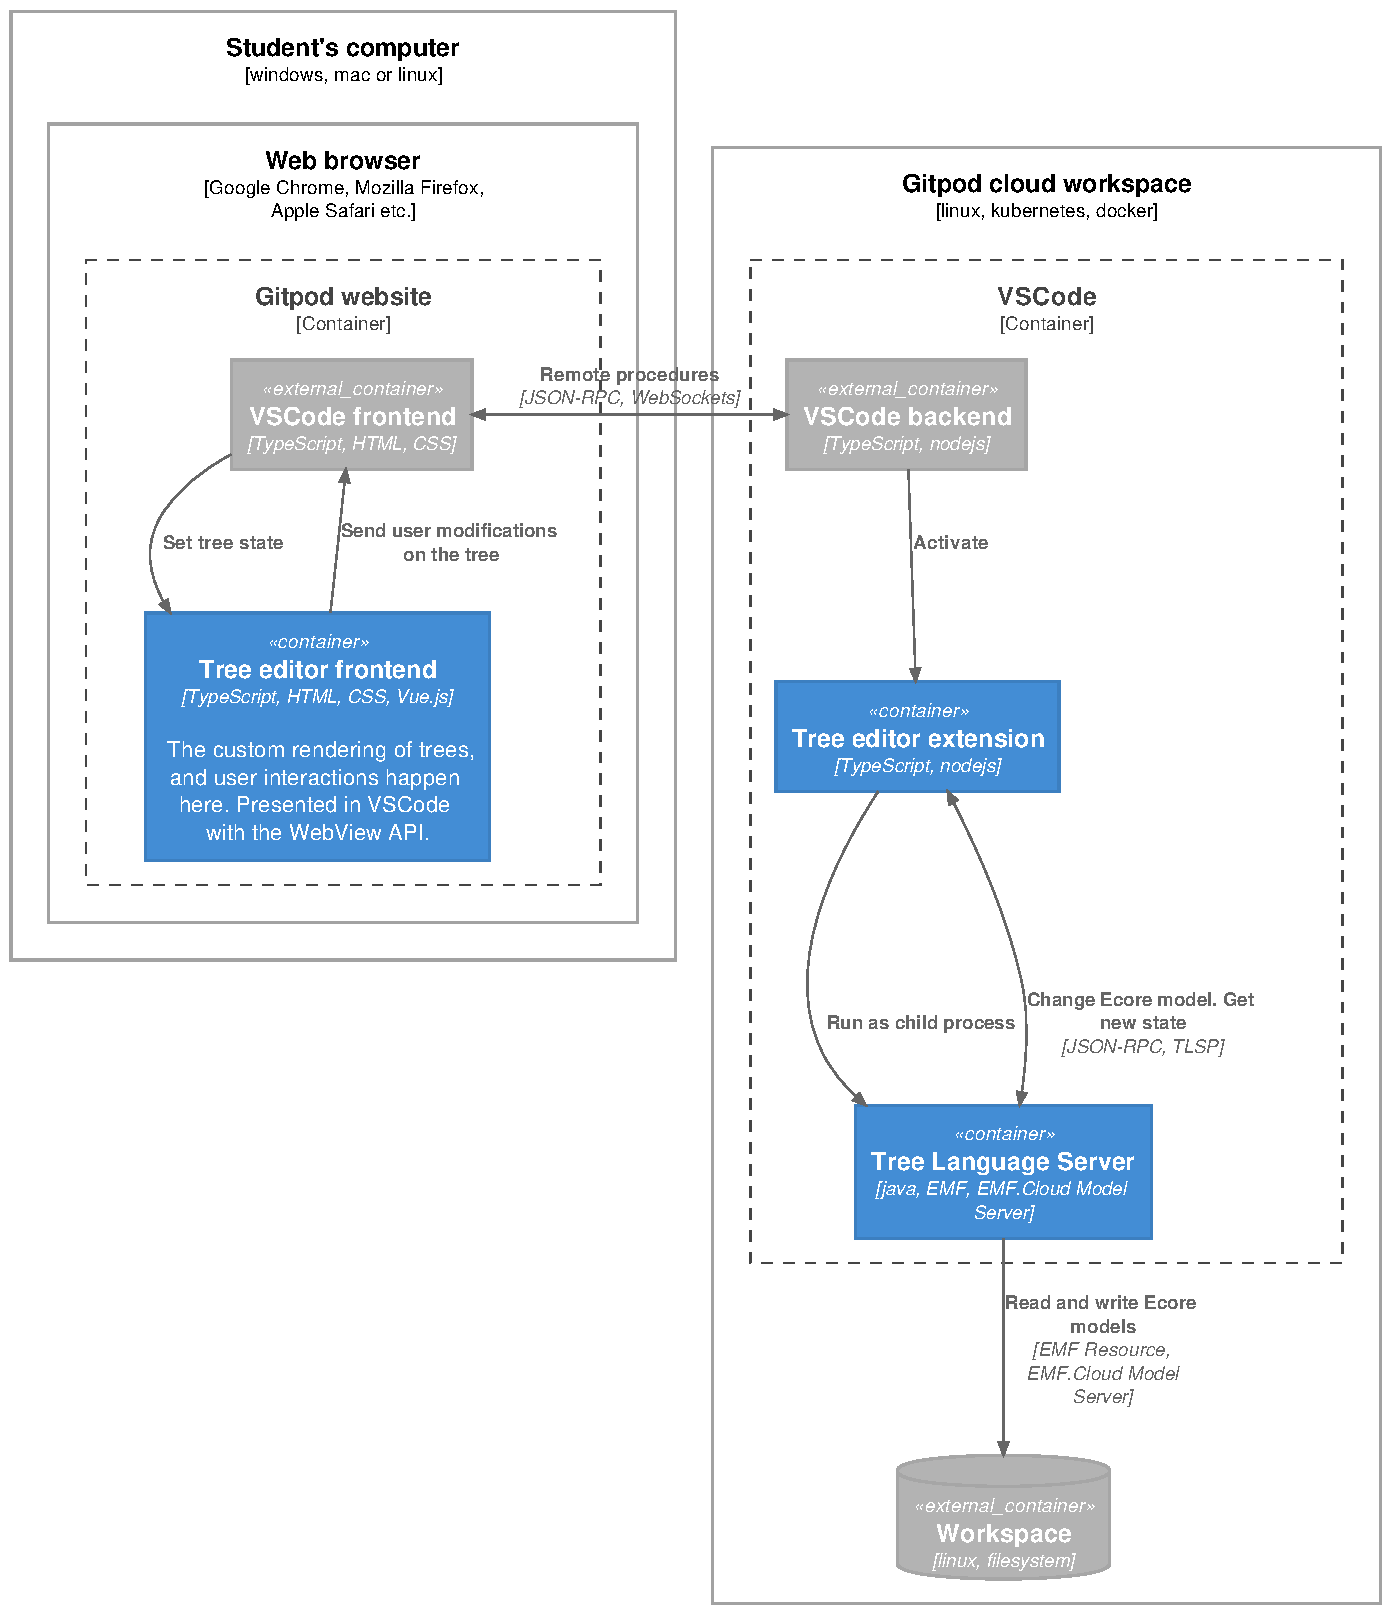
\includegraphics[width=\textwidth,height=\textheight,keepaspectratio]{figures/plantuml/Tree_Editor_Extension_deployment.pdf}
  \caption[Gitpod deployment diagram]{Deployment diagram of Gitpod. The student will use their computer to load the Gitpod website.
  The Gitpod service will start a computer in a cloud provider, to create a cloud workspace.
  The student only loads the VSCode frontend and Tree editor frontend into their browser.
  VSCode has a backend which runs inside the Workspace, and communicates to the frontend over WebSockets, using JSON-RPC\@.
  The VSCode backend will activate the Tree editor extension, which in turn will start a Tree Language Server.
  This Tree Language Server runs java, and reuses the \acrshort{EMF} tooling.
  The Tree editor extension communicates to the Tree Language Server over a well defined protocol, where it asks to read model files, and execute commands to change the models.
  The Tree Language Server uses the Workspace to read and write \texttt{.ecore} files.}\label{fig:gitpod-deployment-diagram}
\end{figure}

The Tree editor extension and Tree Language Server talk together using a protocol named \acrfull{TLSP}.
This protocol is another design artifact from this thesis, and is described later in \cref{sec:tlsp}.
This protocol knows nothing about \acrshort{EMF}, and the same with the Tree editor frontend.
These two parts of the design only work on generic tree structures, as described in \cref{sec:tree-structures}.\\

The Tree editor extension is the component responsible for providing both the Tree editor frontend, and the Tree Language Server.
It also knows about \acrshort{EMF}, because it registers the \texttt{ecore}, \texttt{genmodel} and \texttt{xmi} file extensions to \gls{VSCode} and \gls{Theia}.
The custom Commands from the \acrshort{IDE}'s Command Palette are provided by this Tree editor extension as well.\\

Any changes to the student's model files are saved to disk by the Tree Language Server.
The Tree editor frontend is close to stateless, and the Tree editor extension only bridges the Tree editor frontend and the TLS.

\subsubsection{Code}

\paragraph{Modules}
At a code module level, the Ecore Tree Editor extension is made of 5 modules.
The extension, frontend, server, and two shared libraries: \textit{Tree Document model} and \textit{VSCode and Webview RPC} (or simply RPC library).
The frontend and extension both use the Tree Document model and the RPC library.
This is shown in \cref{fig:extension-code-modules}.
All the modules are coded with \gls{TypeScript}, except the server, which uses Java.\\

The server also ``uses'' the Tree Document model, but by re-implementing\footnote{Not ideal, but no good transpiling (programming language translating) software was found in a reasonable amount of time, to automate this.} it in java.
The Tree Document model module is the result of using Domain Driven Design and a layered architecture (by \textcite{evansDomaindrivenDesignTackling2004}).
It encapsulates the concepts and business logic related to editing tree structures.


\begin{figure}[htbp]  % order of priority: h here, t top, b bottom, p page
  \centering
  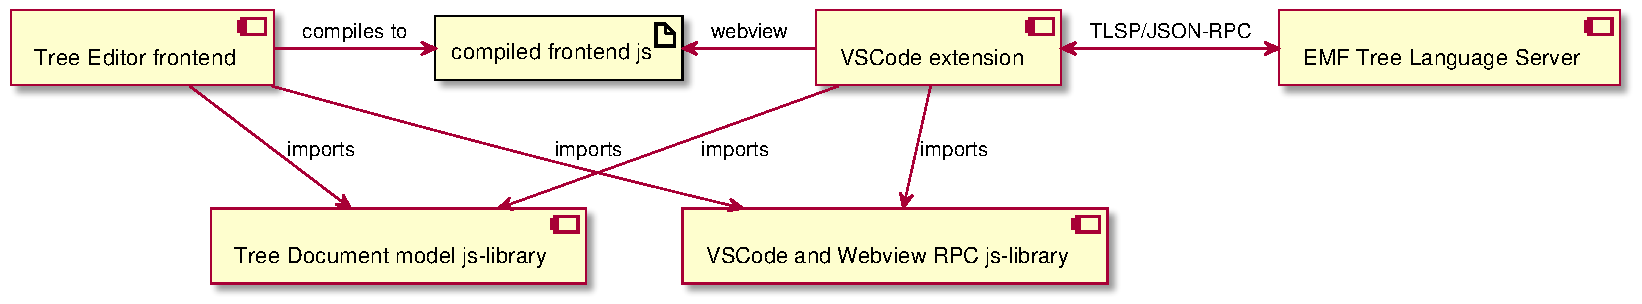
\includegraphics[width=\textwidth]{figures/plantuml/Tree_editor_components.pdf}
  \caption[Ecore Tree Editor component diagram]{Component diagram of the Ecore Tree Editor.
  The for the the extension is organized in 5 separate modules.
  The main module is the VSCode extension.
  This extension bundles the compiled frontend javascript artifact, and the compiled EMF Tree Language Server java jar-file.
  The Tree DOcument model js-library is the layer with the domain model for tree editors.
  It is used in both the frontend and the extension.
  }\label{fig:extension-code-modules}
\end{figure}

\paragraph{Classes}
Three \gls{UML} class diagrams are presented, one each for the frontend, extension and server.
These are not complete, meaning some classes, properties, methods and relationships are not shown.
This is intentional, to increase the clarity, comprehension and the essence of the diagrams.

\paragraph{Frontend classes}
A diagram of the frontend is shown in \cref{fig:tree-editor-frontend-code}.
The execution environment for this is a web browser frame, meaning it has access to the HTML DOM\footnote{Document Object Model, which is how a web browser represents web pages.}.
It has a view layer using a framework called \textit{Vue.js}.
The frontend's state (\texttt{TreeDocument}) is held in a state storage called ``Store'', using a library called \textit{Vuex}.
This state can only be changed through explicit mutations and actions.
This is so the store can intercept changes, and send them to the server via the extension, over the \acrlong{TLSP}.
The frontend talks to the extension using a \texttt{VSCode} interface, where the actual \gls{VSCode} \acrshort{IDE} injects an implementation.
A mocked version (\texttt{MockVSCode}) is provided as an implementation when testing and developing the frontend outside of the \gls{VSCode} \acrshort{IDE}.
Two classes help the communication between the extension and frontend: \texttt{TreeEditorWebview} and \texttt{VscodeExtension}.
These utilize a \gls{JSON-RPC}-like protocol, over the \texttt{VSCode} method called \texttt{postMessage} and the javascript \texttt{Window}'s \texttt{addEventListener}.
The \texttt{FormEditor} view is intended to use the JSON-Forms library, but this view is not finished.

\begin{sidewaysfigure}[htbp]  % order of priority: h here, t top, b bottom, p page
  \centering
  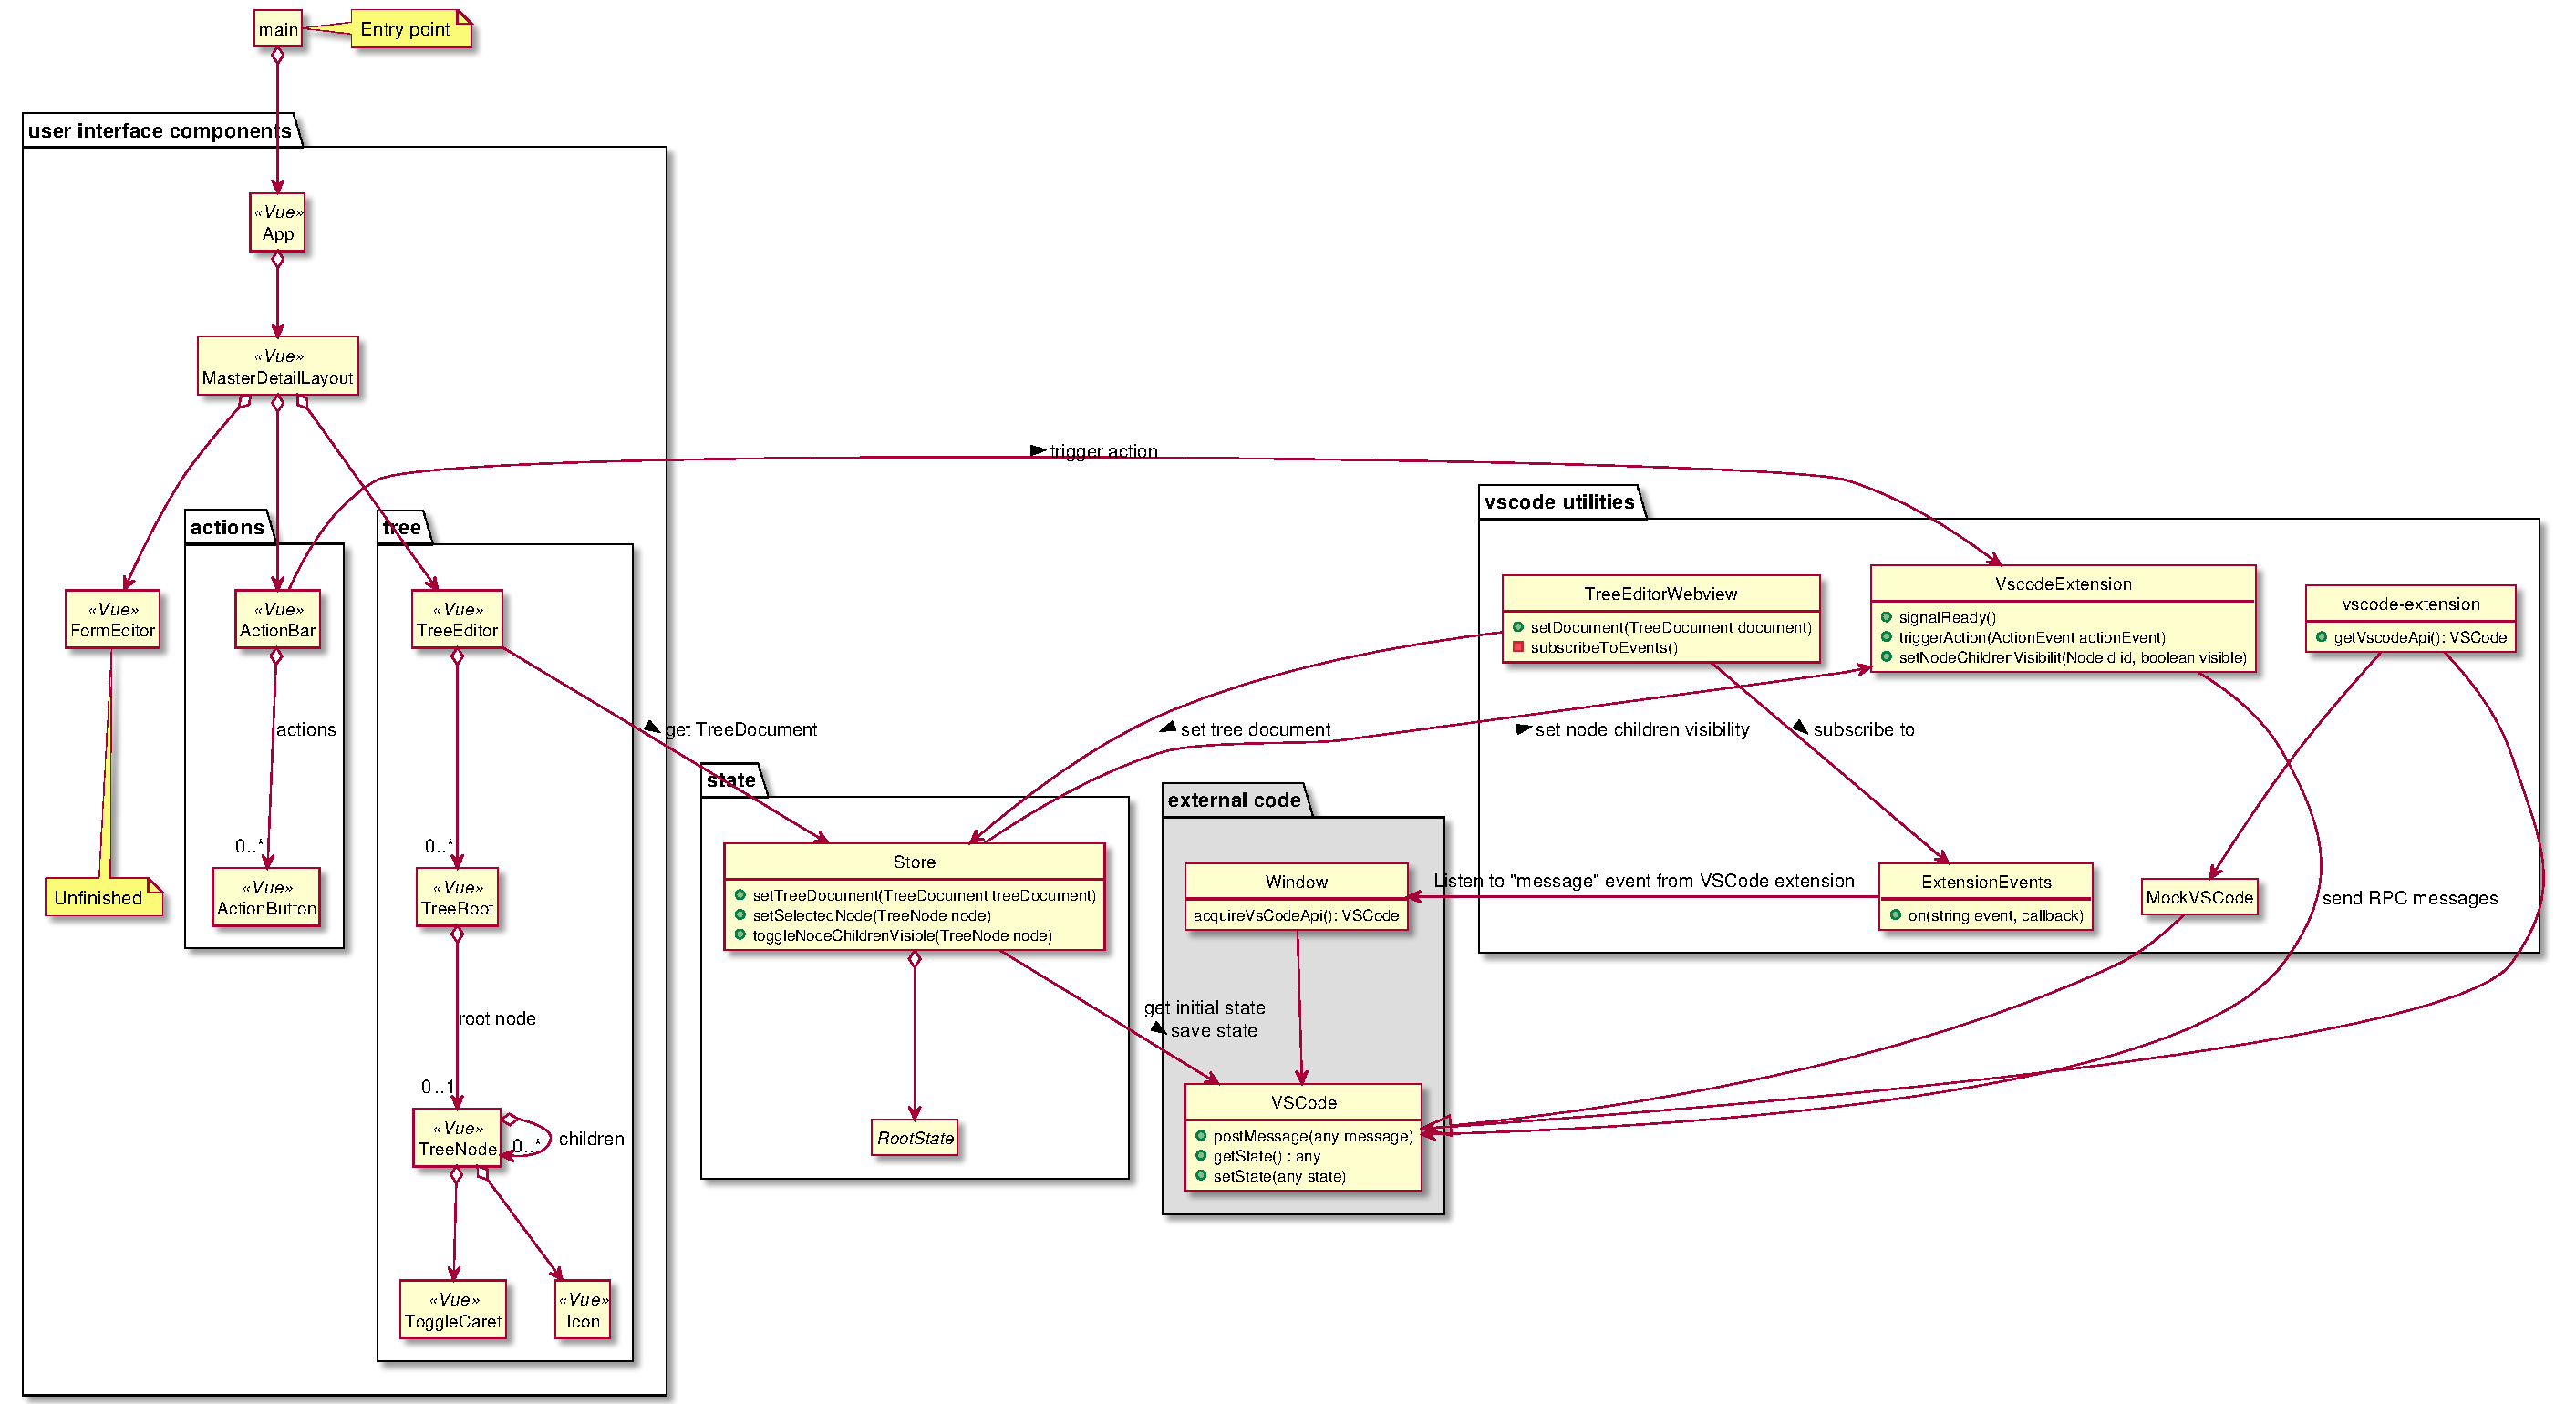
\includegraphics[width=\textwidth,height=1.2\textheight,keepaspectratio]{figures/plantuml/Tree_Editor_Frontend_code.pdf}
  \caption[Tree Editor Frontend class diagram]{Class diagram of the Tree Editor Frontend component.}\label{fig:tree-editor-frontend-code}
\end{sidewaysfigure}

\FloatBarrier

\paragraph{Extension classes}
A diagram of the \gls{VSCode} extension is shown in \cref{fig:tree-editor-extension-code}.
The execution environment for this is \gls{Nodejs}.
The \texttt{extension} file is activated by \gls{VSCode} when particular triggers specified in the extension's \texttt{package.json} manifest occur.
One such trigger is opening a \texttt{.ecore} file.
The \texttt{extension} then registers commands and the custom editor.
The \texttt{CustomTreeEditorProvider} is asked by \gls{VSCode} to create a document and editor for the \texttt{.ecore} file.
The editor uses the compiled outputs of the frontend, and puts it inside a \texttt{WebView}.
A \texttt{WebView} is an isolated execution context provided by \gls{VSCode} (analogous to an \texttt{IFrame} in HTML), where a custom user interface can be shown.
An extension is otherwise not allowed to modify the user interface in \gls{VSCode}.\\

The extension also starts a java process with the executable \texttt{.jar} file for the server.
It then attaches to the \textit{standard in} and \textit{standard out} as communication channels for the \acrshort{TLSP}.
The communication and protocol parsing uses the \texttt{vscode-jsonrpc} library from Microsoft, also used in the official \acrshort{LSP} implementation for \gls{VSCode}.

\begin{sidewaysfigure}[htbp]  % order of priority: h here, t top, b bottom, p page
  \centering
  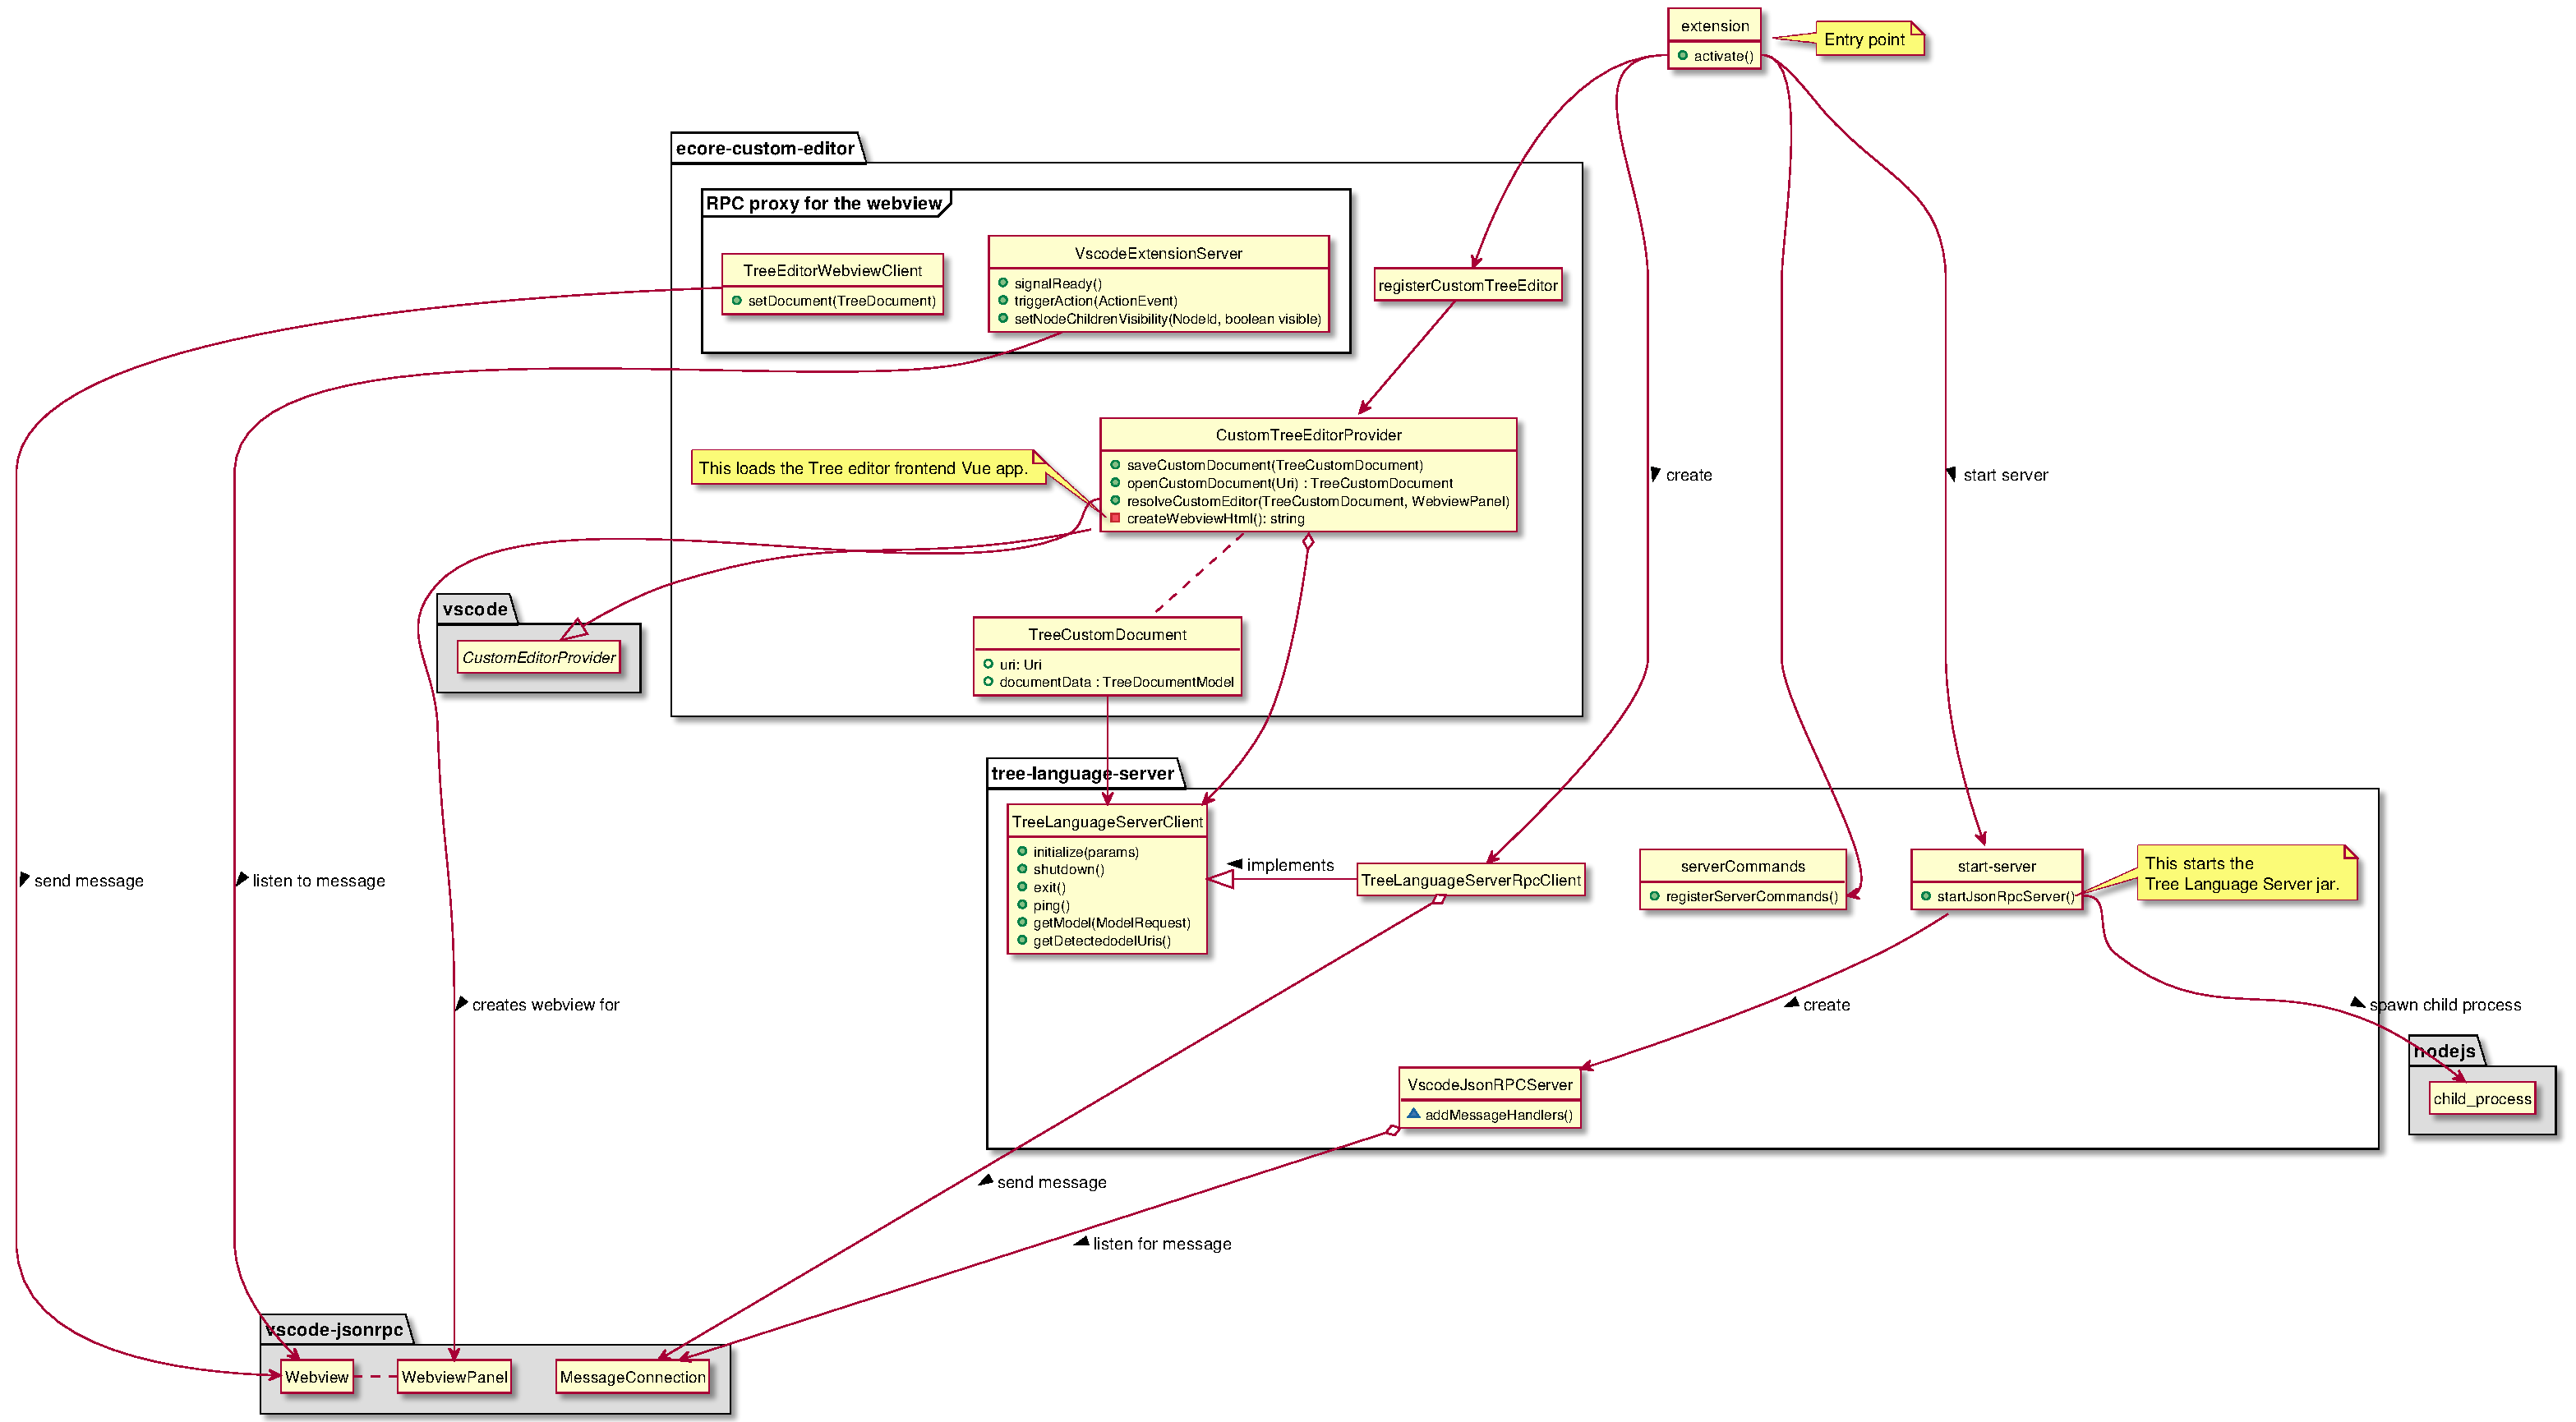
\includegraphics[width=\textwidth,height=1.2\textheight,keepaspectratio]{figures/plantuml/Tree_Editor_Extension_code.pdf}
  \caption[Tree Editor Extension class diagram]{Class diagram of the Tree Editor Extension component.}\label{fig:tree-editor-extension-code}
\end{sidewaysfigure}

\FloatBarrier

\paragraph{Server classes}
A diagram of the server is shown in \cref{fig:tree-editor-server-code}.
The \acrshort{TLSP} server for \acrshort{EMF} starts a \gls{JSON-RPC} server listening to \textit{standard in} and \textit{standard out}, to communicate with the extension.
The protocol is defined with two annotated java interfaces: \texttt{Server} and \texttt{Client}.
The \texttt{Server} represent this server itself, while the \texttt{Client} is the \gls{VSCode} extension side.
An implementation of the \texttt{Server} interface is central, as it does the actual logic in the \acrlong{TLSP}.
The \texttt{ServerImpl} and \texttt{Client} are handed to a \texttt{Launcher}, which comes from the \textit{LSP4J} project.
This is an Eclipse Foundation project which provides a Java \acrshort{LSP}.
Here, the \gls{JSON-RPC} component is standalone, and reused here, with the \acrshort{TLSP} as protocol instead of \acrshort{LSP}.\\

The \texttt{ServerImpl} delegates most of the work to an \texttt{EmfTreeModelController}, which in turn delegates to the EMF.Cloud Model Server or a \texttt{EcoreToTreeDocumentMapper}.
The latter uses the \acrshort{EMF} runtime \acrshort{API} and \texttt{ReflectiveItemProvider} from the \texttt{.edit} \acrshort{EMF} package.
The \texttt{EcoreToTreeDocumentMapper} maps a \acrshort{EMF} \texttt{Resource} to a \texttt{TreeDocument} data structure, compatible with the one in the Tree Document model library component for javascript.

\begin{sidewaysfigure}[htbp]  % order of priority: h here, t top, b bottom, p page
  \centering
  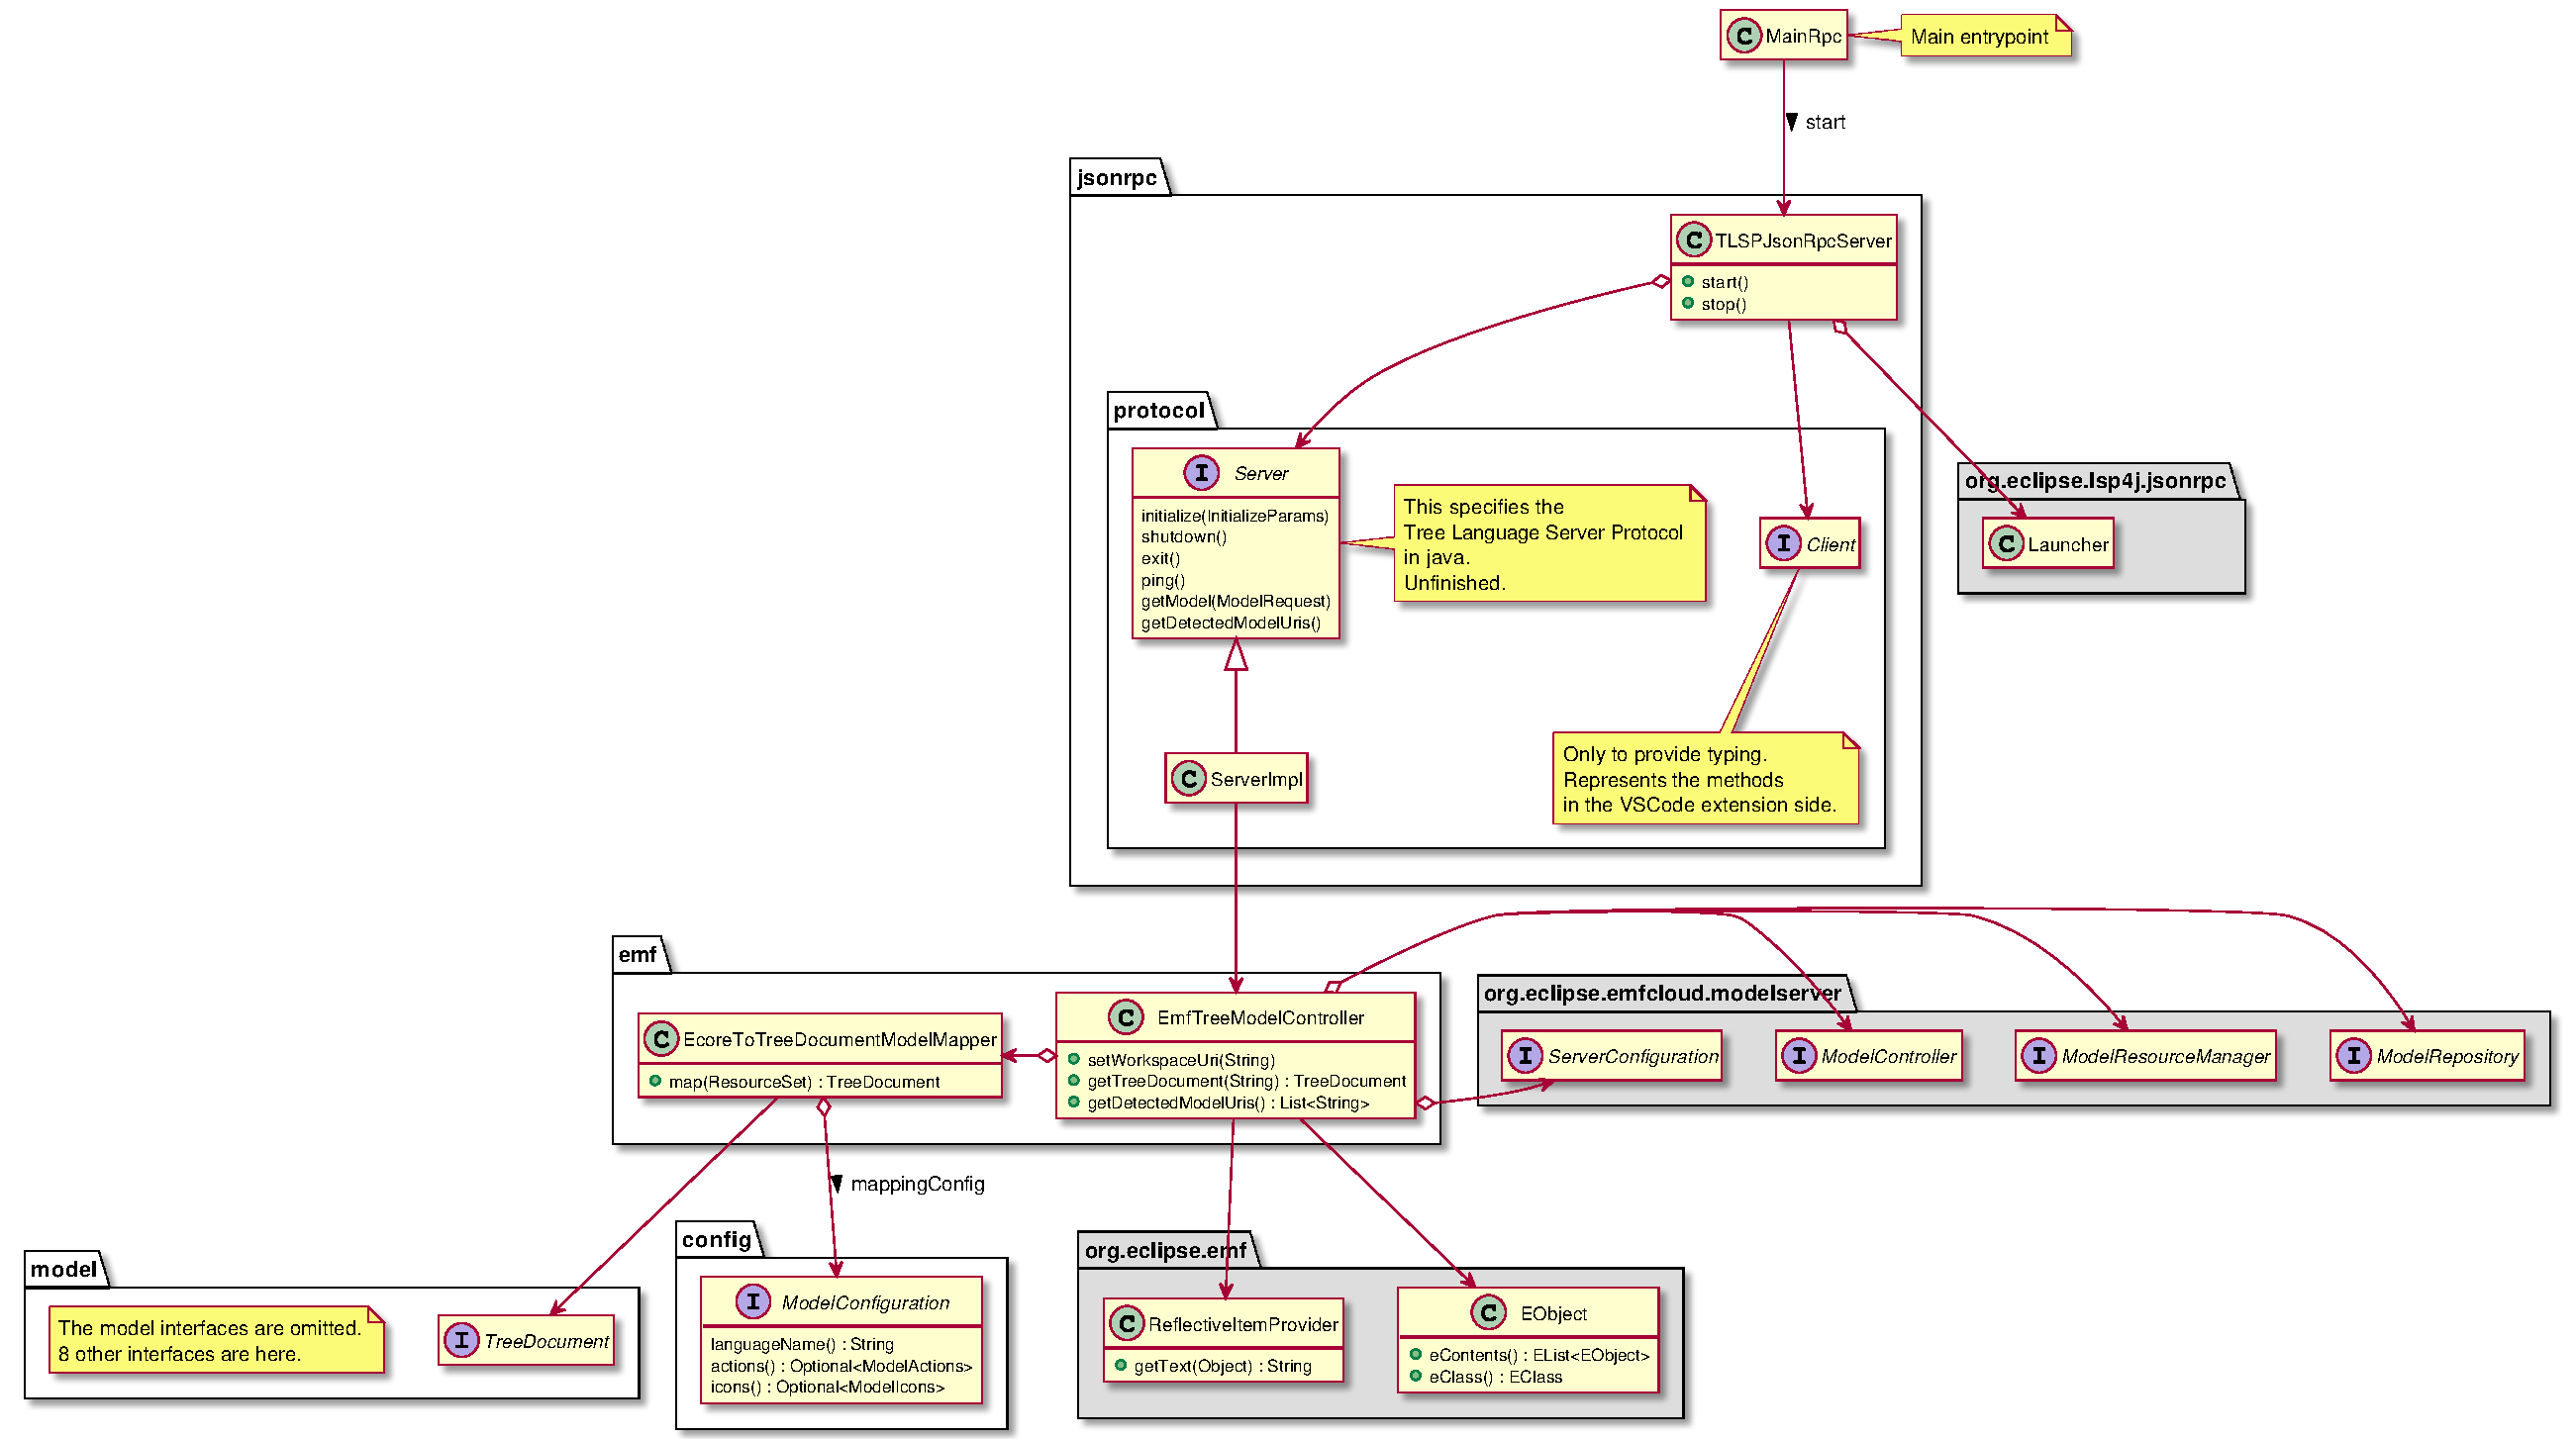
\includegraphics[width=\textwidth,height=\textheight,keepaspectratio]{figures/plantuml/Tree_Language_Server_code.pdf}
  \caption[Tree Language Server class diagram]{Class diagram of the Tree Language Server component.}\label{fig:tree-editor-server-code}
\end{sidewaysfigure}

\FloatBarrier



\section{Design Artifact: Tree Language Server Protocol}\label{sec:tlsp}

\newcommand{\bluearrowDesc}{The blue half-arrow ($\rightharpoondown$) is part of the \acrfull{TLSP}.}

All communication between the Tree Language Server (TLS) and the \gls{VSCode} extension happens over a protocol.
This protocol is part of the artifact design from this thesis, and is called the \acrlong{TLSP}.\\

Because the original \acrshort{EMF} editors are being moved from \gls{Eclipse} to \gls{VSCode}, the protocol draws inspiration from \acrlong{LSP}.
If \gls{Eclipse} already used a \acrshort{LSP}-like language server, the migration would be much easier.
And since it moved once to \gls{VSCode}, it may move again later, for example to IntelliJ (or some other \acrshort{IDE}).\\

The TLSP protocol builds on top the the \textit{Base Protocol} described in \cref{sec:base-protocol}.
That means it sends a header section followed by a content section.
The content has \gls{JSON-RPC} data, being requests, responses, errors, and notifications.
As a reminder: a request must be responded to with a response or error, while a notification does not get an answer.
This means it is a bidirectional communication, where both the extension and the server can initiate a request or notification.
The \acrshort{TLSP} describes what data structures, method names, parameter values and return values should be present in the \gls{JSON-RPC} content.
Because the protocol uses \gls{JSON-RPC} to call the remote procedures, all the data must be serializable to \gls{JSON}.\\

The following subsections present the orders of procedure calls in the \acrshort{TLSP}.
The protocol allows for a stateful server, so for example the workspace must be set before a model is loaded.
The diagrams use UML sequence diagrams.
These have components listed inside boxes at the top, and the timelines as lines coming out below the boxes.
The diagrams are read top to bottom.
A timeline with a box on it represents a process lifetime inside that component.

\subsection{Activation}

Extension activation and document opening is shown in \cref{fig:protocol-startstop}.
When the extension is activated by \gls{VSCode}, the server should be started.
When the server is ready to listen for \acrshort{TLSP} messages, this is indicated by writing a message to an output channel not used for \acrshortpl{TLSP}\footnote{The server uses \textit{standard error} to log and communicate anything that is not \acrshort{TLSP}.}.\\

The extension requests \textit{initialize} with any options the server would need.
The server responds when it is done, allowing the extension to know when it can send the next command.
The workspace path is set to the folder with a student's code.\\

When a \texttt{CustomTreeEditorProvider} in the extension has been asked to open a \texttt{.ecore} document, the server is requested to get the model for this document.
The server responds, and the tree document model is set on the frontend.\\

If the extension is asked to stop, it will first send a \textit{shutdown} request to the server, allowing it to respond when ready to stop.
Then an \textit{exit} notification is sent, which stops the server and breaks the communication.
This shutdown followed by exit procedure is directly inspired by \acrshort{LSP}.


\begin{figure}[htbp]  % order of priority: h here, t top, b bottom, p page
  \centering
  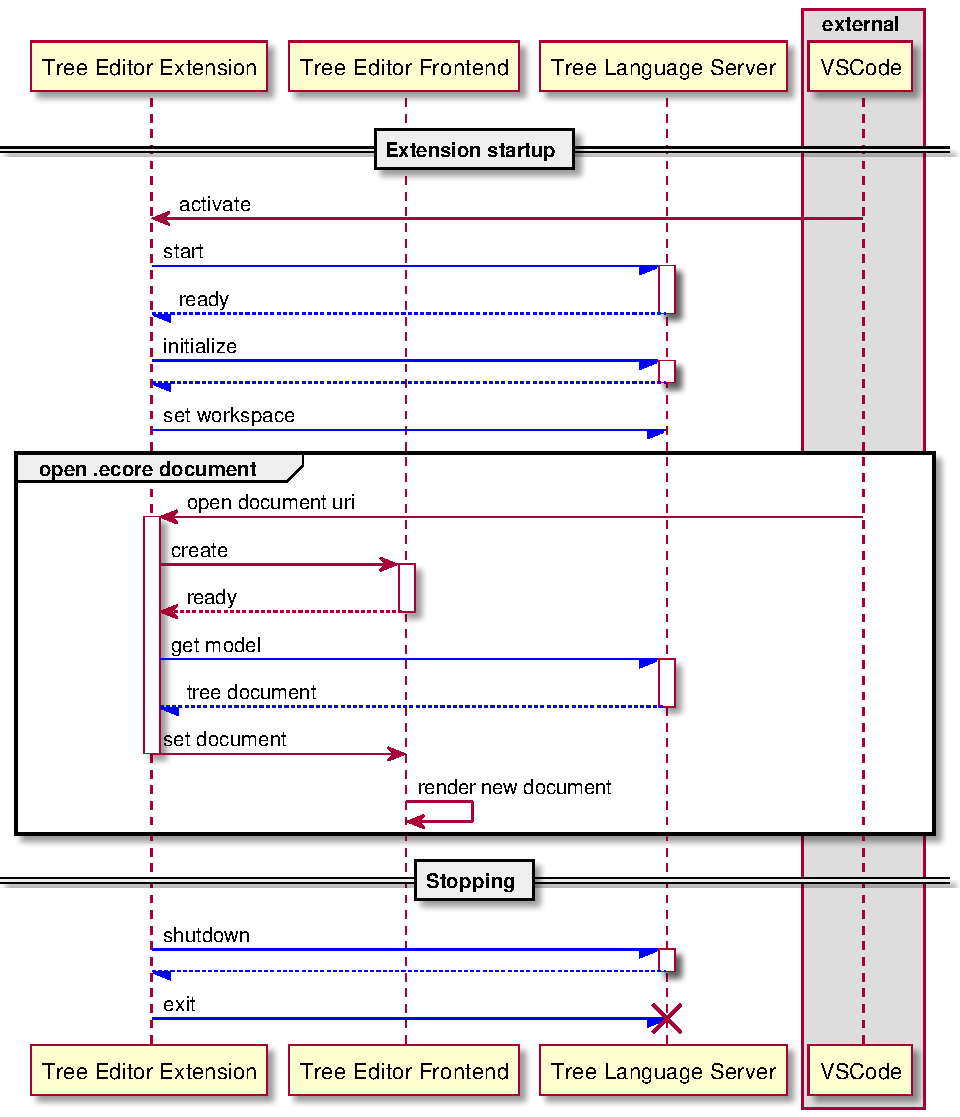
\includegraphics[width=\textwidth]{figures/plantuml/Protocol_startstop_sequence.pdf}
  \caption[Protocol Sequence Diagram of Start/Stop and Document Opening]{Sequence diagram for the protocol when starting and stopping the server. \bluearrowDesc}\label{fig:protocol-startstop}
\end{figure}

\FloatBarrier

\subsection{User Actions}

When a user triggers an action from the frontend, such as validation or code generation, an \texttt{ActionEvent} is sent to the server.
If this event changes the model, a notification will be sent by the server to update the document state.
This is shown in \cref{fig:protocol-action}.

\begin{figure}[htbp]  % order of priority: h here, t top, b bottom, p page
  \centering
  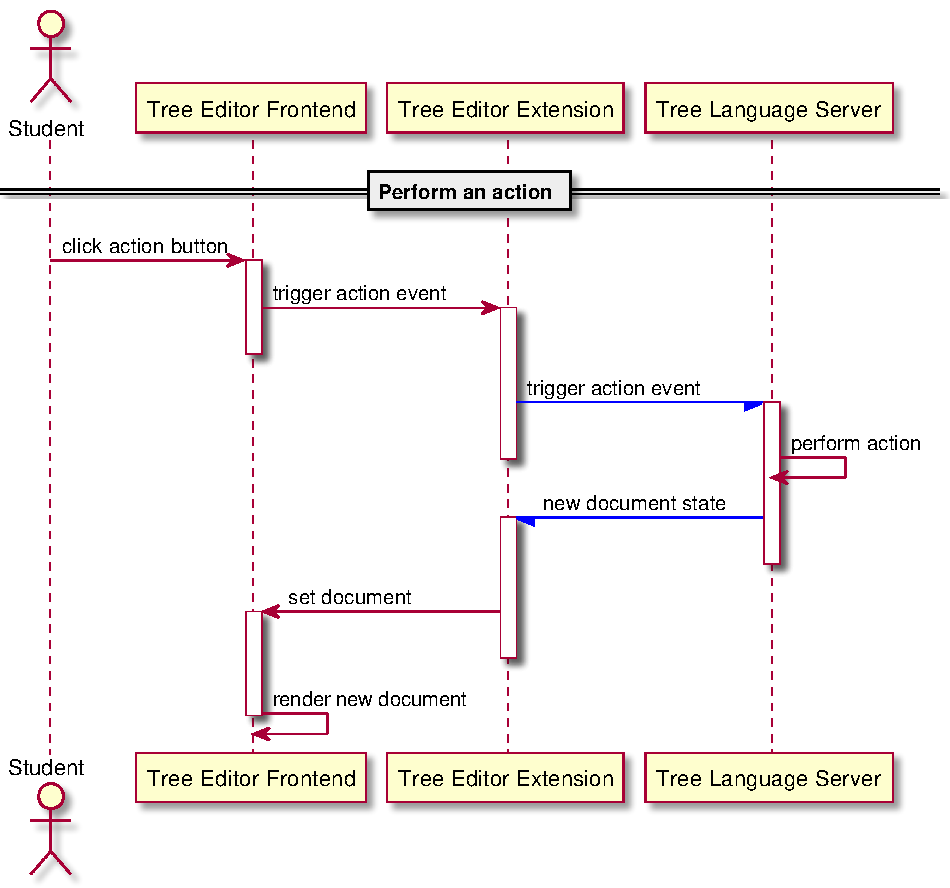
\includegraphics[width=\textwidth]{figures/plantuml/Protocol_action_sequence.pdf}
  \caption[Protocol Sequence Diagram of Action Triggering]{Sequence diagram for the protocol when triggering an action. \bluearrowDesc}\label{fig:protocol-action}
\end{figure}

\FloatBarrier

\subsection{Property Editing}

When a student wants to modify a model element, they first have to select the corresponding tree node.
When the selection changes, the frontend asks the extension for the properties of that node.
This request is then sent to the server, where it returns both the node properties and the schema for JSON-Forms to present it.
This is shown in \cref{fig:protocol-form}.\\

Then when the properties of the node are changed, an event is sent to the server indicating the id of the node and the new property values.
This is shown in the lower half of \cref{fig:protocol-form}.

\begin{figure}[htbp]  % order of priority: h here, t top, b bottom, p page
  \centering
  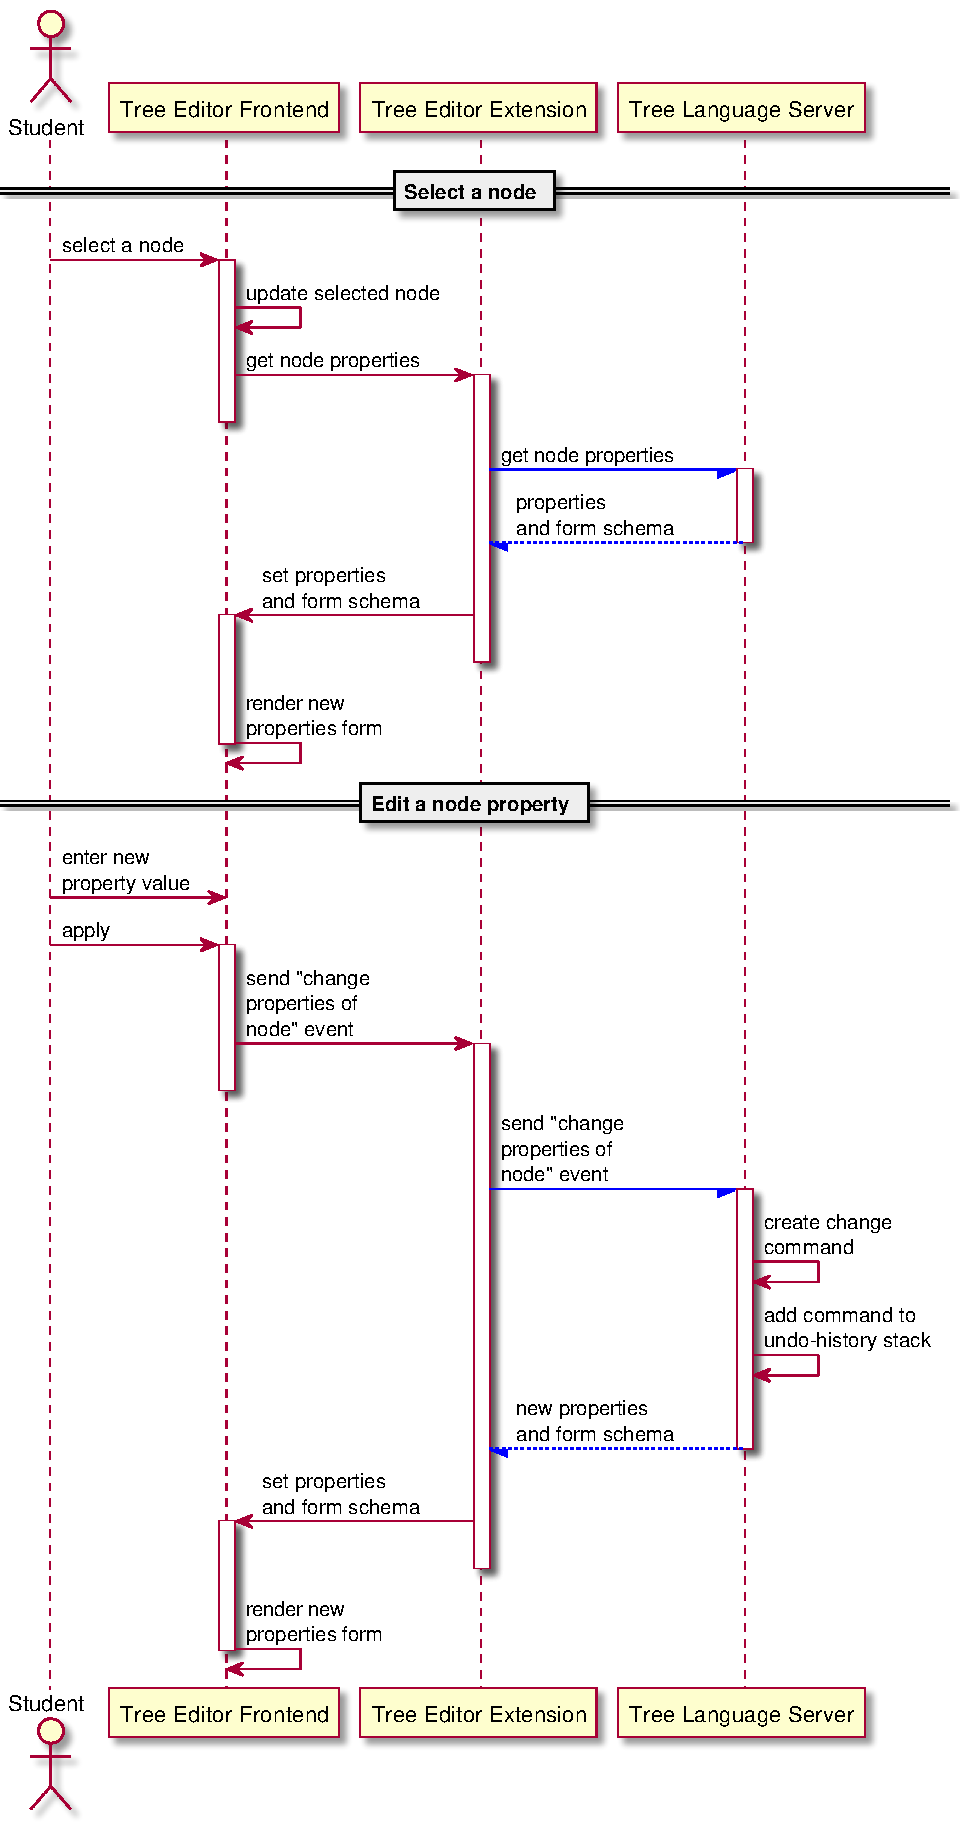
\includegraphics[width=\textwidth,height=\textheight,keepaspectratio]{figures/plantuml/Protocol_form_sequence.pdf}
  \caption[Protocol Sequence Diagram of Property Form]{Sequence diagram for the protocol when editing a node property. \bluearrowDesc}\label{fig:protocol-form}
\end{figure}

\FloatBarrier

\subsection{Tree Editing}

Editing the tree hierarchy by adding children is done by first selecting the child node's type.
This can be presented using the \texttt{HierarchySchema}, which is already sent on the \texttt{TreeDocument} when the model was loaded.
When a student selects the node to add a child on, and the type of child node, this is sent via the extension towards the server.
The server should create a \texttt{Command} from the \texttt{.edit} framework, in order to have a undo/redo history.
The new document state is returned afterwards.
This is shown in \cref{fig:protocol-changetree}.

\begin{figure}[htbp]  % order of priority: h here, t top, b bottom, p page
  \centering
  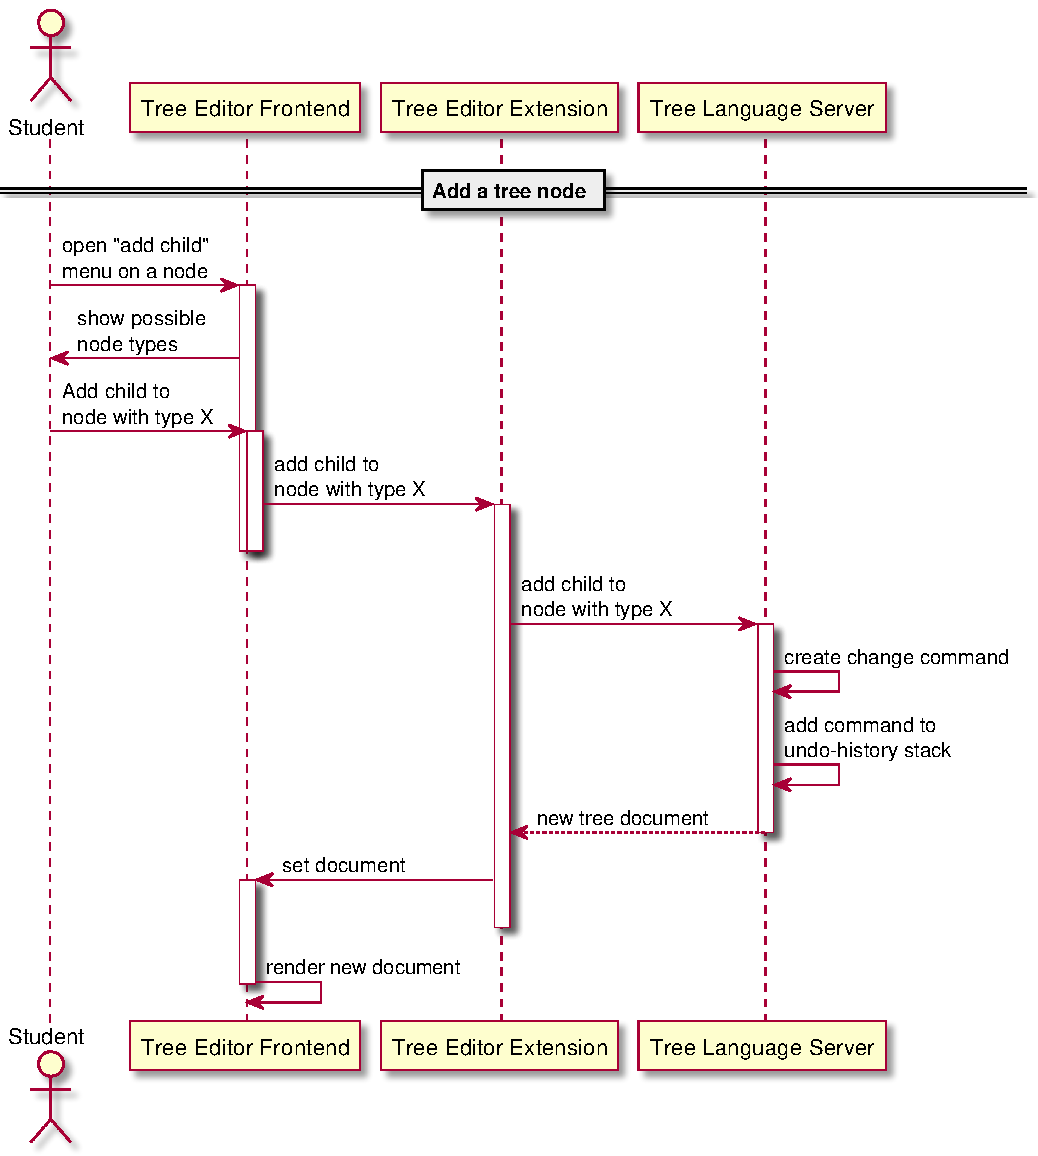
\includegraphics[width=\textwidth]{figures/plantuml/Protocol_changetree_sequence.pdf}
  \caption[Protocol Sequence Diagram of Tree Changes]{Sequence diagram for the protocol when adding a child node. \bluearrowDesc}\label{fig:protocol-changetree}
\end{figure}


\FloatBarrier



\section{Open Source Project: Measures Taken for Viability and Maintainability}


This section will describe the measures taken in order to make the project%
\footnote{The results report on the project in version \texttt{59b722c117}, available at \href{https://github.com/krissrex/tdt4900-master-thesis-ecore-tree-editor/tree/59b722c117346dcc53da16275819e0d5952f0d05}{\nolinkurl{https://github.com/krissrex/tdt4900-master-thesis-ecore-tree-editor/tree/59b722c117346dcc53da16275819e0d5952f0d05}}.}
viable and maintainable as an \gls{open source} project.

\subsection{Code Availability}

Possibly the most important part of \gls{open source}, is available source code.
The project is hosted%
\footnote{Project source: \href{https://github.com/krissrex/tdt4900-master-thesis-ecore-tree-editor}{\nolinkurl{https://github.com/krissrex/tdt4900-master-thesis-ecore-tree-editor}}.}
on a public website for collaboration on \gls{open source} software: \gls{GitHub}.

Also important, is the project visibility being \textit{public}, not private.

The project has the supervisor added as a contributor, in case one project maintainer is unavailable.

\subsection{Documentation}

\paragraph{Readme}
The main project has a ``Readme'' file with an overview of the project's components.

The components named ``tree-document-model-js'', ``tree-editor-frontend'', ``vscode-ecore-tree-editor-extension'' and ``vscode-webview-tree-editor-rpc'' have a Readme.
The ``model-server'' component does not have a Readme.\\

All the readme files are either very minimal, or the default Readme from a project generator.


\paragraph{Source code}
All the modules contain some comments inside the source code.
Not all the source code is documented, only where the author deemed it necessary.
A code base search%
\footnote{
\texttt{
ag --stats -c --ignore-dir dist '\textbackslash{}Q/**\textbackslash{}E\textbackslash{}s' .
}}
returned that 58 files of 169 files had comments, with a total of 128 comments.

\subsection{Automation}

\paragraph{Package manager}
A package manager is used for installing dependencies and compiling each module individually.
For the TypeScript modules, \texttt{npm} (Node Package Manager) is used, and dependencies are tracked in a \texttt{package.json}.
For the java module, \texttt{mvn} (Apache Maven) is used, and dependencies are tracked in a \texttt{pom.xml}.

\paragraph{Build}
Build scripts using \texttt{bash} are provided, that compile the modules (using npm or mvn) and copy the outputs to the correct path.
They also build in the correct order, regarding inter-module dependencies.

\paragraph{IDE configuration}
Files are added to automatically configure a contributor's \acrshort{IDE}, if they use \gls{VSCode} for the TypeScript modules and IntelliJ for the java module.
When using \gls{VSCode}, a list of recommended extensions is provided as well, which can be automatically installed.
There are \textit{Tasks} defined for \gls{VSCode} that can trigger the different npm builds, and \textit{Run configurations} to start the modules.

\paragraph{CI/CD}
There is no Continuous Integration (CI) and Continuous Deployment (CD) configured.
This can be added later when needed; for 1 developer it is overhead.

\subsection{Licensing}

\paragraph{Module license}
The modules use the MIT license\footnote{https://opensource.org/licenses/MIT}.
It is a very simple and permissive license, compatible with \gls{open source}, and commonly used.
The licenses are not in separate files or the readme.
They are instead mentioned in the \texttt{package.json} and \texttt{pom.xml} files.

\paragraph{Copied code}
Some code is copied from other sources.
The original license has been included in these cases.
No code is copied from incompatible or strict licenses that contradict MIT.

\paragraph{Third party dependencies}
No proprietary dependencies are used%
\footnote{TypeScript modules were scanned with: \lstinline{npx license-checker --production}.}
, and none with incompatible or intrusive licenses.

\subsection{Code}

\paragraph{Code style}
The code uses readable names and small files.
The programming languages (TypeScript and Java) are common, especially in this context.
The code is formatted with automatic code formatters\footnote{Prettier and IntelliJ format the code.}, ensuring a consistent style.

\paragraph{Dependencies}
The dependencies and libraries used are common and in some cases official, in this context.
Effort has been put into using the same dependencies as related works (such as \acrshort{LSP} and EMF.Cloud projects).


\subsection{Issue Tracking}

An issue tracker is available on \gls{GitHub}.
A user is required, but signup is free.
A discussion forum is available as well on \gls{GitHub}.
There is no Wiki, but it is easy to create one on \gls{GitHub} if demand arises.


